\documentclass[xcolor=svgnames,9pt,english, aspectratio=169]{beamer}
%\documentclass[xcolor=svgnames,9pt,english, handout, aspectratio=169]{beamer}
\newcommand{\handout}{0}
% Shared template layer for the six decks: theme, beamer layout, and the packages
% every deck needs. Each deck inputs this near the top of its preamble, BEFORE
% ../common/theme.tex (metropolis must be selected before the palette overrides it).
%
% Notation macros and theorem environments are deliberately NOT shared. They
% conflict between the decks, and merging them would silently change symbols
% inside equations:
%   \e          decks 1-2: \bs{\epsilon}      deck 3: \boldsymbol{\eta}
%   \M          decks 1-2: \mb{M}             deck 3: \mathcal{M}
%   \blue       decks 1-2: blue               deck 3: RoyalBlue
%   \indep      different implementations
%   assumption / proposition
%               decks 1-2: own counter        deck 3: shares the theorem counter
%
% Each deck therefore keeps its own notation block. Only the look is unified.

\usetheme{metropolis}
\setbeamertemplate{navigation symbols}{}

% Deck 3's margins; decks 1 and 2 previously used 2em, which at 9pt is ~6.3mm.
\setbeamersize{text margin left=5mm, text margin right=5mm}
\setbeamertemplate{itemize/enumerate body begin}{\leftmargini=1.5em\relax}
\setbeamertemplate{itemize/enumerate subbody begin}{\leftmarginii=1.5em\relax}
\setbeamertemplate{itemize/enumerate subsubbody begin}{\leftmarginiii=1.5em\relax}

\usepackage{xcolor}
\usepackage{colortbl}
\usepackage{amsmath}
\usepackage{amsfonts}
\usepackage{amssymb}
\usepackage{graphicx}
\usepackage{multirow}
\usepackage{listings}
\usepackage{booktabs}
\usepackage{tikz}
\usetikzlibrary{arrows.meta,positioning,decorations.pathreplacing}

% Citations: one bib file at the repository root, Chicago author-date via biblatex-chicago
% (needs biber). Reference frames are generated with \printbibliography; in-text citations
% use \textcite (narrative) and \parencite (parenthetical). The CMS rule prints one to three
% names in full and four or more as "First et al."; \citeshort forces "et al.", \citeall
% prints every name (text/paren/author variants likewise). The override lasts one citation.
\usepackage{csquotes}
\usepackage[authordate,backend=biber,doi=false,url=false,isbn=false,eprint=false,
            maxbibnames=10,compresspages=true,dashed=false]{biblatex-chicago}
\addbibresource{../references.bib}
% Entry size: beamer wraps each part of a biblatex entry in its "bibliography entry author /
% title / location / note" fonts, and metropolis sets those to \normalsize, so \bibfont alone
% does not change the size. The four \setbeamerfont lines in theme.tex set the size that shows.
\renewcommand*{\bibfont}{\scriptsize}
\setlength{\bibitemsep}{0.7em}   % visible air between entries
\setlength{\bibhang}{0.5em}
% The References frame of every deck: \begin{frame}[t,allowframebreaks=1.0] ... \referencelist.
% Beamer's automatic break for this list fires at about two thirds of the frame; the factor
% 1.1 lets it fill the frame. The small negative skip closes the list's top gap.
\newcommand{\referencelist}{\vspace*{-0.6em}\printbibliography[heading=none]}
\newcommand{\citeshort}[1]{\AtNextCitekey{\defcounter{maxnames}{1}}\cite{#1}}
\newcommand{\textciteshort}[1]{\AtNextCitekey{\defcounter{maxnames}{1}}\textcite{#1}}
\newcommand{\parenciteshort}[1]{\AtNextCitekey{\defcounter{maxnames}{1}}\parencite{#1}}
\newcommand{\citeauthorshort}[1]{\AtNextCitekey{\defcounter{maxnames}{1}}\citeauthor{#1}}
\newcommand{\citeall}[1]{\AtNextCitekey{\defcounter{maxnames}{9}}\cite{#1}}
\newcommand{\textciteall}[1]{\AtNextCitekey{\defcounter{maxnames}{9}}\textcite{#1}}
\newcommand{\parenciteall}[1]{\AtNextCitekey{\defcounter{maxnames}{9}}\parencite{#1}}
% PDF metadata: beamer copies the whole \author box into the author field; set it plainly
% once every deck-level \author has run (etoolbox's end-of-preamble hook).
\AtEndPreamble{\hypersetup{pdfauthor={Yiqing Xu}}}
   % theme, layout, packages

\setbeamertemplate{footline}[frame number]{}

\graphicspath{{./figs/}}%
\newcommand{\red}{\textcolor{red}}

\usepackage{epsfig}
\usepackage{makecell}
\usetikzlibrary{decorations.pathreplacing,calc}
% Shared visual system for the six decks: palette, fonts, footline.
% Swap the four colors below to rebrand every deck at once.
\definecolor{SlideRed}{HTML}{9E1B32}
\definecolor{SlideInk}{HTML}{252A34}
\definecolor{SlideBlue}{HTML}{2F6B9A}
\definecolor{SlideMist}{HTML}{F8F3F3}


\setbeamercolor{normal text}{fg=SlideInk,bg=white}
\setbeamercolor{structure}{fg=SlideRed}
\setbeamercolor{alerted text}{fg=SlideRed}
\setbeamercolor{frametitle}{fg=white,bg=SlideRed}
\setbeamercolor{title}{fg=SlideRed}
\setbeamercolor{subtitle}{fg=SlideInk}
\setbeamercolor{block title}{fg=white,bg=SlideRed}
\setbeamercolor{block body}{fg=SlideInk,bg=SlideMist}
\setbeamercolor{section in toc}{fg=SlideRed}

\setbeamerfont{title}{series=\bfseries,size=\Large}
\setbeamerfont{frametitle}{series=\bfseries,size=\large}
\setbeamerfont{block title}{series=\bfseries}
\setbeamertemplate{navigation symbols}{}
\setbeamertemplate{items}[circle]
\setbeamertemplate{blocks}[rounded][shadow=false]
\setbeamertemplate{bibliography item}{}   % no document icons on the References frames
\setbeamertemplate{frametitle continuation}{}
\setbeamertemplate{footline}{%
  \leavevmode\hbox{%
  \begin{beamercolorbox}[wd=.88\paperwidth,ht=2.6ex,dp=1.2ex,leftskip=1.2em]{author in head/foot}%
  \usebeamerfont{author in head/foot}\insertshorttitle
  \end{beamercolorbox}%
  \begin{beamercolorbox}[wd=.12\paperwidth,ht=2.6ex,dp=1.2ex,center]{date in head/foot}%
  \insertframenumber
  \end{beamercolorbox}}}

\newcommand{\slidesource}[1]{\vfill{\scriptsize\color{gray}Source: #1}}
\newcommand{\keyquestion}[1]{\begin{block}{Question}#1\end{block}}


\title{Panel Methods (3): Factorial Difference-in-Differences}
\subtitle{Lectures on Causal Panel Analysis}
\author{Yiqing Xu\\\smallskip Stanford University}
\date{September 2026}

% ---------- notation (deck-local; do not merge across decks) ----------
\newcommand{\E}{\ensuremath{\mathbb{E}}}
\newcommand{\indep}{{\perp\!\!\!\perp}}
\newcommand{\tdid}{\ensuremath{\tau_{\mathrm{DID}}}}
\newcommand{\tdidhat}{\ensuremath{\hat{\tau}_{\mathrm{DID}}}}
\newcommand{\tem}{\ensuremath{\tau_{\mathrm{em}}}}
\newcommand{\tcm}{\ensuremath{\tau_{\mathrm{cm}}}}
\newcommand{\tatt}{\ensuremath{\tau_{\mathrm{att}}}}
\newcommand{\tgz}{\ensuremath{\tau_{G|Z=1}}}

% ---------- deck-local drawing helpers ----------
% The two Clans-and-Calamity maps are cropped from the original slides with one shared box; the
% bullets reach into that box, so white tikz rectangles (fractions detected from the crops) cover the leaked text.
\definecolor{gridLight}{HTML}{E9EEF6}
\definecolor{gridDark}{HTML}{4472C4}
% Two-group event figure, drawn with a fixed bounding box so overlays never shift.
% #1 title  #2 G=1 label  #3 G=0 label  #4 Delta for G=1  #5 Delta for G=0
% #6 brace/annotation text (empty = none; if #4 = #5 the text is placed without a brace)
% #7 mode: f = factorial view (red counterfactuals + Delta labels); z = same, G=0's label reads Delta = 0; c = canonical view
\newcommand{\twogroupfig}[7]{%
\begin{tikzpicture}[x=0.9cm, y=0.75cm, >=Latex]
\useasboundingbox (-1.0,-1.0) rectangle (6.2,6.4);
\pgfmathsetmacro{\yOneCf}{2.6+0.7}\pgfmathsetmacro{\yZeroCf}{0.8+0.7}
\pgfmathsetmacro{\yOne}{\yOneCf+#4}\pgfmathsetmacro{\yZero}{\yZeroCf+#5}\pgfmathsetmacro{\yRef}{\yOneCf+#5}
\draw[->, thick] (-0.3,0) -- (5.3,0) node[below left=1pt] {\scriptsize Time};
\draw[->, thick] (-0.3,0) -- (-0.3,5.4) node[left=1pt] {\scriptsize $Y$};
\node[below=2pt] at (0,0) {\scriptsize Pre};\node[below=2pt] at (4,0) {\scriptsize Post};
\node[above] at (2.3,5.7) {\small #1};
\if#7c\else
  \draw[red, densely dotted] (0,2.6) -- (4,\yOneCf);\draw[red] (4,\yOneCf) circle (1.4pt);
  \draw[red, densely dotted] (0,0.8) -- (4,\yZeroCf);\draw[red] (4,\yZeroCf) circle (1.4pt);
\fi
\draw[thick] (0,0.8) -- (4,\yZero);\fill (0,0.8) circle (1.6pt);\fill (4,\yZero) circle (1.6pt);
\draw[thick] (0,2.6) -- (4,\yOne);\fill (0,2.6) circle (1.6pt);\fill (4,\yOne) circle (1.6pt);
\node[anchor=south east, inner sep=1pt] at (2.7,{2.6+0.675*(\yOne-2.6)+0.12}) {\scriptsize #2};
\node[anchor=north west, inner sep=1pt] at (2.0,{0.8+0.5*0.7-0.12}) {\scriptsize #3};
\if#7c\else
  % Delta labels: none on the same-U frames (Delta_1 = Delta_0); upper Delta sits between the reference point and the
  % counterfactual point when the DID reference is drawn; none when Delta_0 = 0 or in the canonical view
  \if#7z\else\ifdim #4pt=#5pt\else
    \ifx\\#6\\\else\node[right=2pt] at (4,{(\yOneCf+\yRef)/2}) {\scriptsize $\Delta$};\fi\fi\fi
  \if#7z\node[right=2pt, red] at (4,\yZeroCf) {\scriptsize $\Delta = 0$};\else\ifdim #4pt=#5pt\else\node[right=2pt] at (4,{(\yZeroCf+\yZero)/2}) {\scriptsize $\Delta$};\fi\fi
\fi
\ifx\\#6\\\else
  \ifdim #4pt=#5pt
    \node[right=4pt] at (4,\yOne) {\scriptsize #6};
  \else
    \draw[densely dotted] (0,2.6) -- (4,\yRef);\draw (4,\yRef) circle (1.4pt);
    \draw[decorate, decoration={brace, amplitude=4pt}] (4.45,\yOne) -- (4.45,\yRef) node[midway, right=5pt] {\scriptsize #6};
  \fi
\fi
\end{tikzpicture}}
\newcommand{\pre}{\mathrm{pre}}

% ---------- paper cards for the "More Examples" frames (deck-local) ----------
% \papercard{width}{authors and year}{venue}{title}{one-line design}
\newcommand{\papercard}[5]{%
\begin{tikzpicture}
\node[draw=SlideRed, thick, rounded corners=3pt, fill=SlideMist, inner sep=8pt, text width=#1, align=left] {%
  {\small\textbf{#4}}\\[0.45em]
  {\footnotesize #2. \emph{#3}.}\\[0.6em]
  {\footnotesize\color{SlideInk}#5}};
\end{tikzpicture}}
\newcommand{\post}{\mathrm{post}}

% ---------- potential-outcome tree (deck-local) ----------
% \potree{0} = plain tree; \potree{1} = with tau braces
\newcommand{\potree}[1]{%
\begin{tikzpicture}[x=1cm,y=1cm, font=\footnotesize]
\node[font=\footnotesize\bfseries] at (3.35,3.0) {Pre-Event};
\node[font=\footnotesize\bfseries] at (5.15,3.0) {Post-Event};
\node (root) at (0.1,0) {Unit $i$};
\draw[densely dotted, thick] (0.55,0.15) -- (1.55,1.65);
\draw[densely dotted, thick] (0.55,-0.15) -- (1.55,-1.65);
\node at (0.72,1.22)  {$g=1$};
\node at (0.72,-1.22) {$g=0$};
\draw[densely dotted, thick] (1.6,1.75) -- (2.45,2.3);
\draw[densely dotted, thick] (1.6,1.75) -- (2.45,1.15);
\draw[densely dotted, thick] (1.6,-1.75) -- (2.45,-1.2);
\draw[densely dotted, thick] (1.6,-1.75) -- (2.45,-2.35);
\node at (1.95,2.25)  {$z=1$};
\node at (1.95,1.15)  {$z=0$};
\node at (1.95,-1.2)  {$z=1$};
\node at (1.95,-2.35) {$z=0$};
\node at (3.35,2.35)  {$Y_{i,\pre}(1,1)$};
\node[red] at (3.35,1.15)  {$Y_{i,\pre}(1,0)$};
\node at (3.35,-1.2)  {$Y_{i,\pre}(0,1)$};
\node[red] at (3.35,-2.35) {$Y_{i,\pre}(0,0)$};
\node at (5.15,2.35)  {$Y_{i,\post}(1,1)$};
\node[red] at (5.15,1.15)  {$Y_{i,\post}(1,0)$};
\node at (5.15,-1.2)  {$Y_{i,\post}(0,1)$};
\node[red] at (5.15,-2.35) {$Y_{i,\post}(0,0)$};
\if#11
\draw[decorate,decoration={brace,amplitude=4pt}] (5.95,2.5) -- (5.95,1.0)
  node[midway,right=5pt] {$\tau_{i,Z|G=1}$};
\draw[decorate,decoration={brace,amplitude=4pt}] (5.95,-1.05) -- (5.95,-2.5)
  node[midway,right=5pt] {$\tau_{i,Z|G=0}$};
\draw[decorate,decoration={brace,amplitude=5pt}] (7.6,2.0) -- (7.6,-2.0)
  node[midway,right=6pt] {$\tau_{i,\mathrm{cm}}$};
\fi
\end{tikzpicture}}

% ---------- identification roadmap (deck-local) ----------
% \idmap{0} = roadmap version (only tau_DID = tau_em); \idmap{1} = complete map
\newcommand{\idmap}[1]{%
\begin{tikzpicture}[x=1cm,y=1cm, font=\footnotesize, align=center]
\node (tdid) at (0,0)    {\LARGE $\tdid$};
\node (tem)  at (4.9,0)  {\LARGE $\tem$};
\node (tcm)  at (9.8,0)  {\LARGE $\tcm$};
\node (tatt) at (4.9,-3.1) {\LARGE $\tatt$};
\node (tgz)  at (9.8,-3.1) {\LARGE $\tgz$};
\node[below=2pt of tdid] {A statistical estimand\\consistently estimated by $\tdidhat$};
\node[below=2pt of tem]  {An associative estimand\\describing \alert{effect heterogeneity}};
\node[below=2pt of tcm]  {A causal estimand\\targeting \alert{causal moderation}};
\node[below=2pt of tatt] {A causal estimand targeting\\the effect of $Z$ for $G=1$};
\node[below=2pt of tgz]  {A causal estimand targeting\\the effect of $G$ when $Z=1$};
\draw[double distance=2pt, thick] (1.2,0) -- (3.7,0)
  node[midway, above=3pt] {No anticipation \&\\parallel trends};
\if#11
\draw[double distance=2pt, thick] (6.1,0) -- (8.6,0)
  node[midway, above=3pt] {$\Delta Y(g,z) \indep G$\\(factorial parallel trends)};
\draw[double distance=2pt, thick] (4.9,-1.0) -- (4.9,-2.4)
  node[midway, left=4pt] {Exclusion restriction\\on $Z$ for $G=0$};
\draw[double distance=2pt, thick] (9.8,-1.0) -- (9.8,-2.4)
  node[midway, left=4pt] {Exclusion restriction\\on $G$ absent the event};
\fi
\end{tikzpicture}}

\begin{document}

\AtBeginSection[]
{
  \begin{frame}<beamer>
    \frametitle{Outline}
    \tableofcontents[currentsection]
  \end{frame}
}

\begin{frame}
  \titlepage
  \thispagestyle{empty}
  \addtocounter{framenumber}{-1}
\end{frame}

\begin{frame}
  \frametitle{The Six Lectures}
\begin{center}
\begin{tikzpicture}[
  lecture/.style={rounded corners=3pt, draw=SlideRed, thick,
                  minimum height=1.6cm, text width=2.6cm,
                  align=center, inner sep=5pt},
  link/.style={-{Latex[length=2.2mm]}, thick, draw=SlideInk}
]
\node[lecture, fill=SlideMist] (l1) at (0,0)
  {\textbf{1. Parametric panel models}\\[0.25em]
   \footnotesize FE regressions and their assumptions};
\node[lecture, fill=SlideMist] (l2) at (0,-2.9)
  {\textbf{2. Difference-in-differences}\\[0.25em]
   \footnotesize The canonical design and identification};
\node[lecture, fill=SlideRed!25, very thick] (l3) at (3.9,0)
  {\textbf{3. Factorial DID}\\[0.25em]
   \footnotesize When the event affects everyone};
\node[lecture, fill=SlideMist] (l4) at (3.9,-2.9)
  {\textbf{4. TWFE revisited}\\[0.25em]
   \footnotesize What breaks under staggered timing};
\node[lecture, fill=SlideMist] (l5) at (7.8,0)
  {\textbf{5. Modern DID}\\[0.25em]
   \footnotesize Heterogeneity-robust estimators};
\node[lecture, fill=SlideMist] (l6) at (7.8,-2.9)
  {\textbf{6. Synthetic control \& factor models}\\[0.25em]
   \footnotesize Imputing treated counterfactuals};
\draw[link] (l1) -- (l2);
\draw[link] (l2.east) -- ++(0.5,0) |- (l3.west);
\draw[link] (l3) -- (l4);
\draw[link] (l4.east) -- ++(0.5,0) |- (l5.west);
\draw[link] (l5) -- (l6);
\end{tikzpicture}
\end{center}
\end{frame}

\begin{frame}
  \frametitle{Where We Are}
\begin{itemize}[<+->]\itemsep1em
\item Lecture 2 covered the canonical DID design: a treated group, an untreated comparison group, and parallel trends
\item But many events leave \alert{no one untreated}: a famine, a financial crisis, a pandemic, a nationwide reform
\item Applied work still runs ``DID'' in these settings, comparing units that differ in a \alert{pre-event characteristic}
\item This lecture: what does that comparison identify, and under which assumptions? (\cite{xu2026factorial}, \emph{JASA})
\item Lecture 4 then returns to TWFE regressions and what breaks under staggered timing
\end{itemize}
\end{frame}

\section{Motivation}

\begin{frame}[t]
  \frametitle{Motivation: How Social Capital Saved Lives}
\begin{columns}[T,onlytextwidth]
\begin{column}{0.5\textwidth}
\begin{itemize}\itemsep0.6em
\item \alert{\textcite{cao2022clans}}: ``How social capital saved lives during China's Great Famine''
\item<2-> Data structure:
\begin{itemize}\itemsep0.3em
  \item<3-> A baseline factor $G$: time-invariant measure of social capital
  \item<3-> Event time: \{Pre-Famine, Famine, Post-Famine\}
\end{itemize}
\item<5-> Estimation: difference-in-differences (DID), or equivalently, two-way fixed effects (TWFE)
\item<7-> Interpretation:
\begin{itemize}\itemsep0.3em
  \item<7-> \alert{Descriptively}: ``the rise in the mortality rate during the famine years is significantly smaller in counties with higher social capital''
  \item<8-> \alert{Causally}: ``we interpret these differences as the effects of social capital on famine relief''
\end{itemize}
\end{itemize}
\end{column}
\begin{column}{0.47\textwidth}
\centering
\only<2-3| handout:0>{%
\begin{tikzpicture}[x=1.35cm, y=1.3cm, >=Latex]
\useasboundingbox (-2.05,-0.8) rectangle (3.1,2.55);
\fill[gridLight] (0,0) rectangle (3,2);
\fill[gridDark] (1,0) rectangle (2,2);
\foreach \c in {1,2} {\draw[white, line width=2pt] (\c,0) -- (\c,2);}
\draw[white, line width=2pt] (0,1) -- (3,1);
\foreach \c/\l in {0/Pre-Famine, 1/Famine, 2/Post-Famine} {\node[above=3pt] at ({\c+0.5},2) {\footnotesize \l};}
\node[left=4pt] at (0,1.5) {\footnotesize Social capital: high};
\node[left=4pt] at (0,0.5) {\footnotesize Social capital: low};
\draw[->, thick] (0,-0.3) -- (3,-0.3) node[midway, below=2pt] {\footnotesize Time};
\end{tikzpicture}}%
\only<4-5| handout:0>{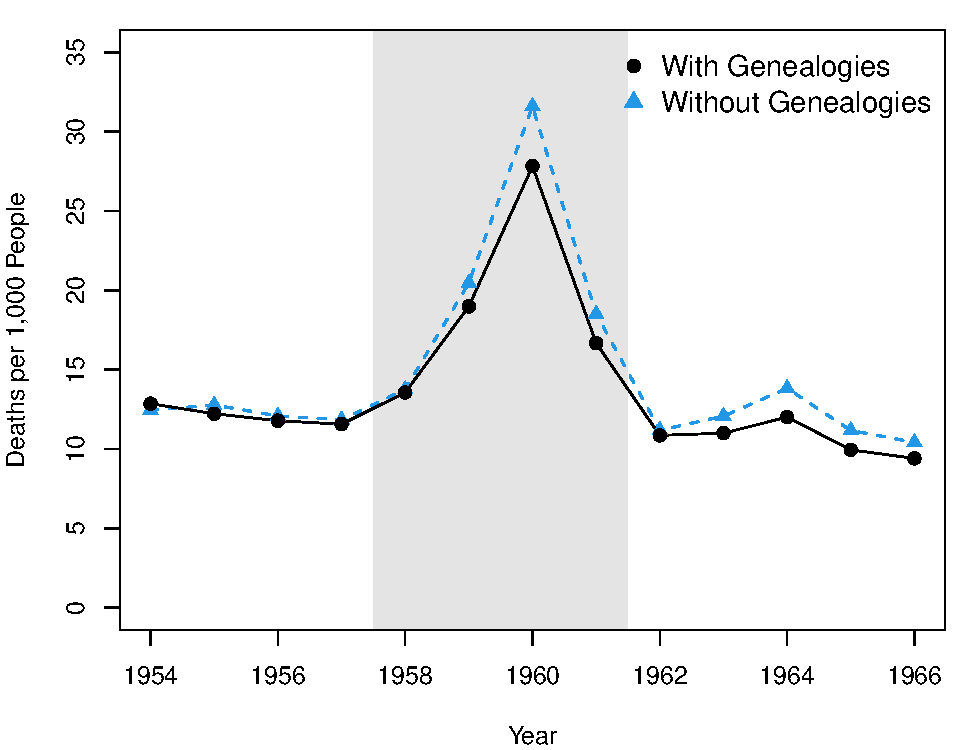
\includegraphics[width=\linewidth, height=0.62\textheight, keepaspectratio]{raw.pdf}
\par{\scriptsize Raw data: mortality by level of social capital.}}%
\only<6-| handout:1>{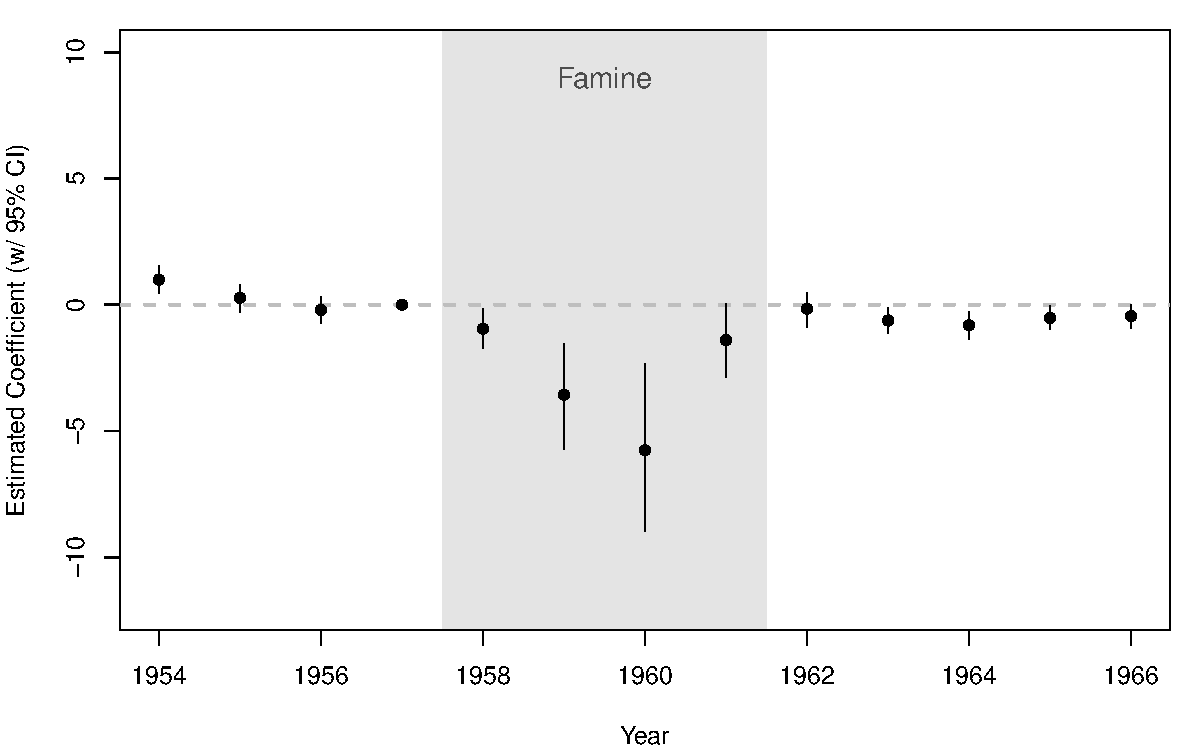
\includegraphics[width=\linewidth, height=0.62\textheight, keepaspectratio]{fig5.pdf}
\par{\scriptsize Estimates from TWFE with a dynamic specification.}}
\end{column}
\end{columns}
\end{frame}

\begin{frame}
  \frametitle{More Examples}
\begin{center}
\papercard{0.8\textwidth}{Vasiliki Fouka (2019)}{American Political Science Review 113 (2)}{How Do Immigrants Respond to Discrimination? The Case of Germans in the US During World War I}{German immigrants (the baseline factor) meet the wave of anti-German hostility that came with the war (the event); outcomes are naming choices and petitions for naturalization.}
\par\medskip{\small\onslide<2->{\alert{Discrimination $\times$ WWI}}}
\end{center}
\slidesource{\textcite{fouka2019how}.}
\end{frame}

\begin{frame}
  \frametitle{More Examples}
\begin{center}
\papercard{0.8\textwidth}{Mara P. Squicciarini (2020)}{American Economic Review 110 (11)}{Devotion and Development: Religiosity, Education, and Economic Progress in Nineteenth-Century France}{More and less religious districts (the baseline factor) meet the Second Industrial Revolution's demand for technical schooling (the event); outcomes are education and industrial development.}
\par\medskip{\small\onslide<2->{\alert{Catholicism $\times$ Industrial Revolution}}}
\end{center}
\slidesource{\textcite{squicciarini2020devotion}.}
\end{frame}

\begin{frame}
  \frametitle{More Examples}
\begin{columns}[b,onlytextwidth]
\begin{column}{0.48\textwidth}
\centering
\papercard{0.92\linewidth}{Joy Chen, Erik H. Wang, and Xiaoming Zhang (2025)}{American Journal of Political Science 69 (2)}{From Powerholders to Stakeholders: State-Building with Elite Compensation in Early Medieval China}{Localities with and without entrenched powerholders meet a state-building reform that reached everyone.}
\par\smallskip{\small\onslide<2->{\alert{Elite strongholds $\times$ state-building reform}}}
\end{column}
\begin{column}{0.48\textwidth}
\centering
\papercard{0.92\linewidth}{Daniel de Kadt and Horacio A. Larreguy (2018)}{Journal of Politics 80 (2)}{Agents of the Regime? Traditional Leaders and Electoral Politics in South Africa}{Areas with and without traditional leaders meet the rise of Jacob Zuma as ANC leader; the outcome is the ANC's vote share.}
\par\smallskip{\small\onslide<3->{\alert{Traditional leaders $\times$ rise of Zuma}}}
\end{column}
\end{columns}
\bigskip
\begin{itemize}
\item<4-> In each study: a \alert{baseline factor $G$} interacted with an \alert{event $Z$ that hits every unit}
\end{itemize}
\slidesource{\textcite{chen2025powerholders}; \textcite{dekadt2018agents}.}
\end{frame}

\begin{frame}
  \frametitle{Same DID Estimator, a Different Research Design}
\begin{center}
\begin{tikzpicture}
\node[rounded corners=8pt, fill=SlideMist, draw=SlideInk, inner sep=10pt, align=center]
  {Same DID estimator, a different research design:\\[0.3em]
   {\Large\bf ``Factorial Difference-in-Differences''}};
\end{tikzpicture}
\end{center}
\bigskip
\begin{columns}[T,onlytextwidth]
\begin{column}{0.48\textwidth}
\begin{itemize}\itemsep0.5em
\item \textbf{Factorial}
\begin{itemize}\itemsep0.4em
  \item A classic topic in statistics
  \item Factorial experiments pioneered by R.~A. Fisher and Frank Yates
  \item $\geq 2$ treatment factors: their main effects and interaction are of interest
\end{itemize}
\end{itemize}
\end{column}
\begin{column}{0.48\textwidth}
\begin{itemize}\itemsep0.5em
\item<2-> \textbf{Difference-in-differences}
\begin{itemize}\itemsep0.4em
  \item<2-> Popular in economics and related fields
  \item<2-> A ``research design'' for causal inference with observational data
  \item<2-> Leverages panel data (units $\times$ time) to identify causal effects, usually the ATT
\end{itemize}
\end{itemize}
\end{column}
\end{columns}
\end{frame}

\begin{frame}[t]
  \frametitle{This Lecture}
\begin{columns}[T,onlytextwidth]
\begin{column}{0.55\textwidth}
\begin{itemize}[<+->]\itemsep1em
\item Factorial DID is a different \underline{research design} from a canonical DID
\item Under no anticipation \& parallel trends, the DID \underline{estimator} identifies \alert{treatment effect heterogeneity} of exposure to the event (with nuances)
\item Identifying $G$'s \alert{causal effect} requires stronger assumptions
\item Factorial DID includes canonical DID as a special case with an additional assumption
\item Extensions \& practical recommendations
\end{itemize}
\end{column}
\begin{column}{0.42\textwidth}
\centering
\only<1| handout:0>{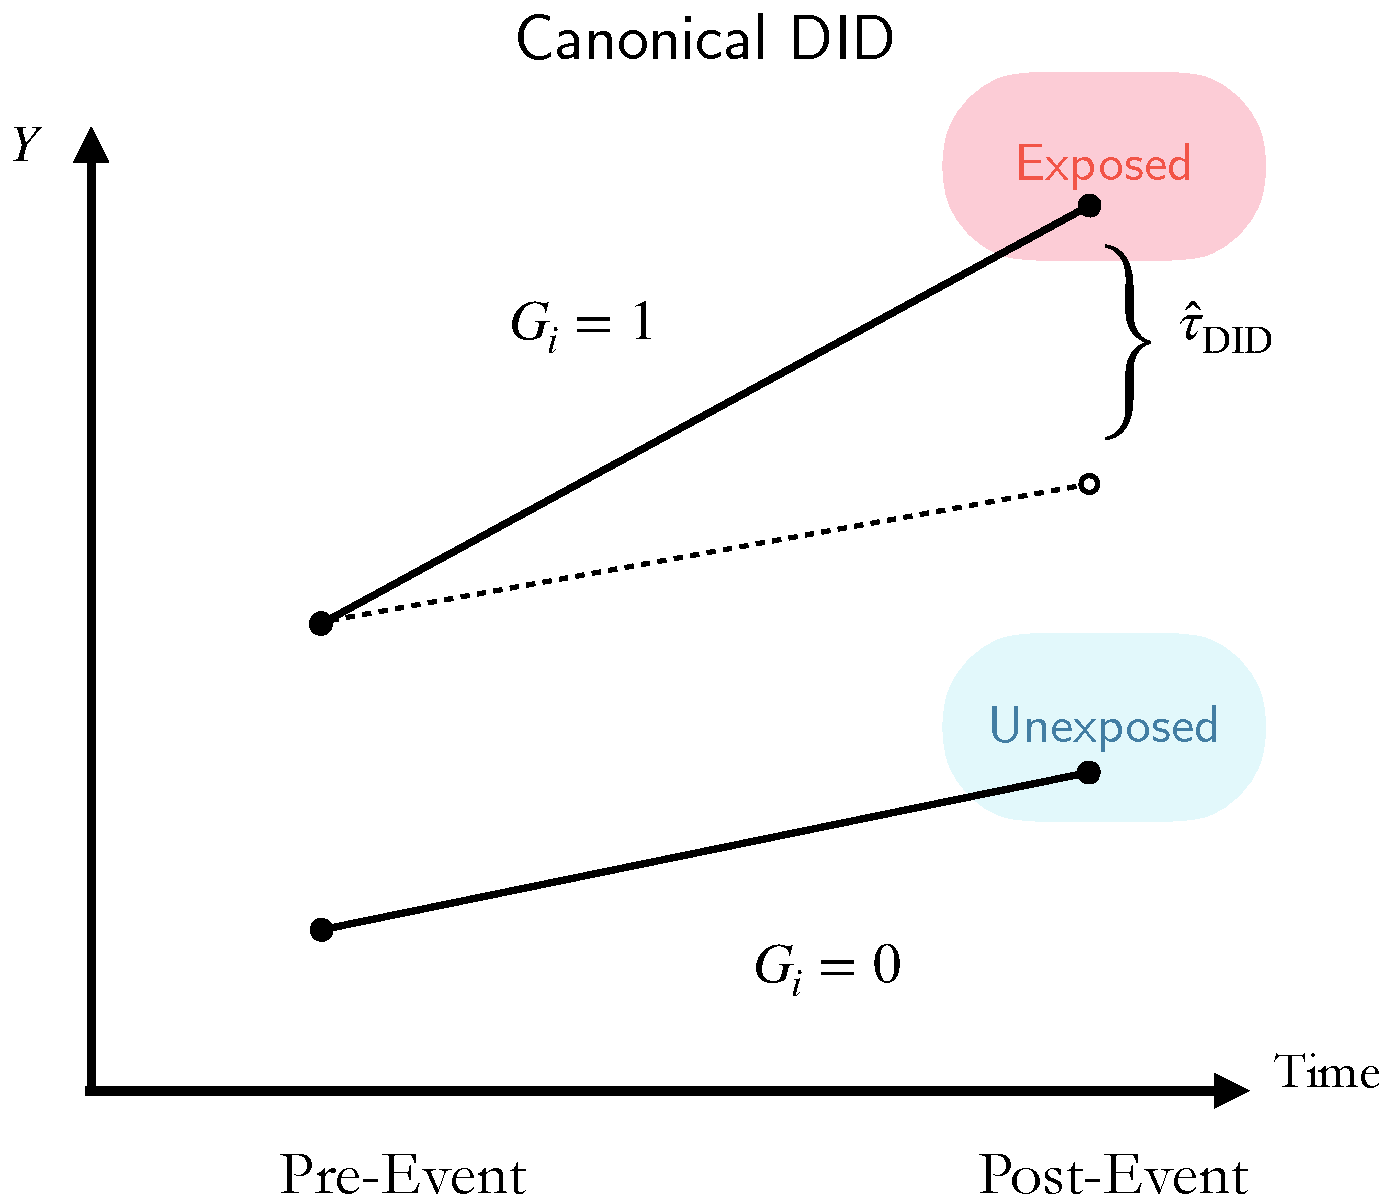
\includegraphics[width=\linewidth, height=0.6\textheight, keepaspectratio]{c_canonical_did.pdf}}%
\only<2-| handout:1>{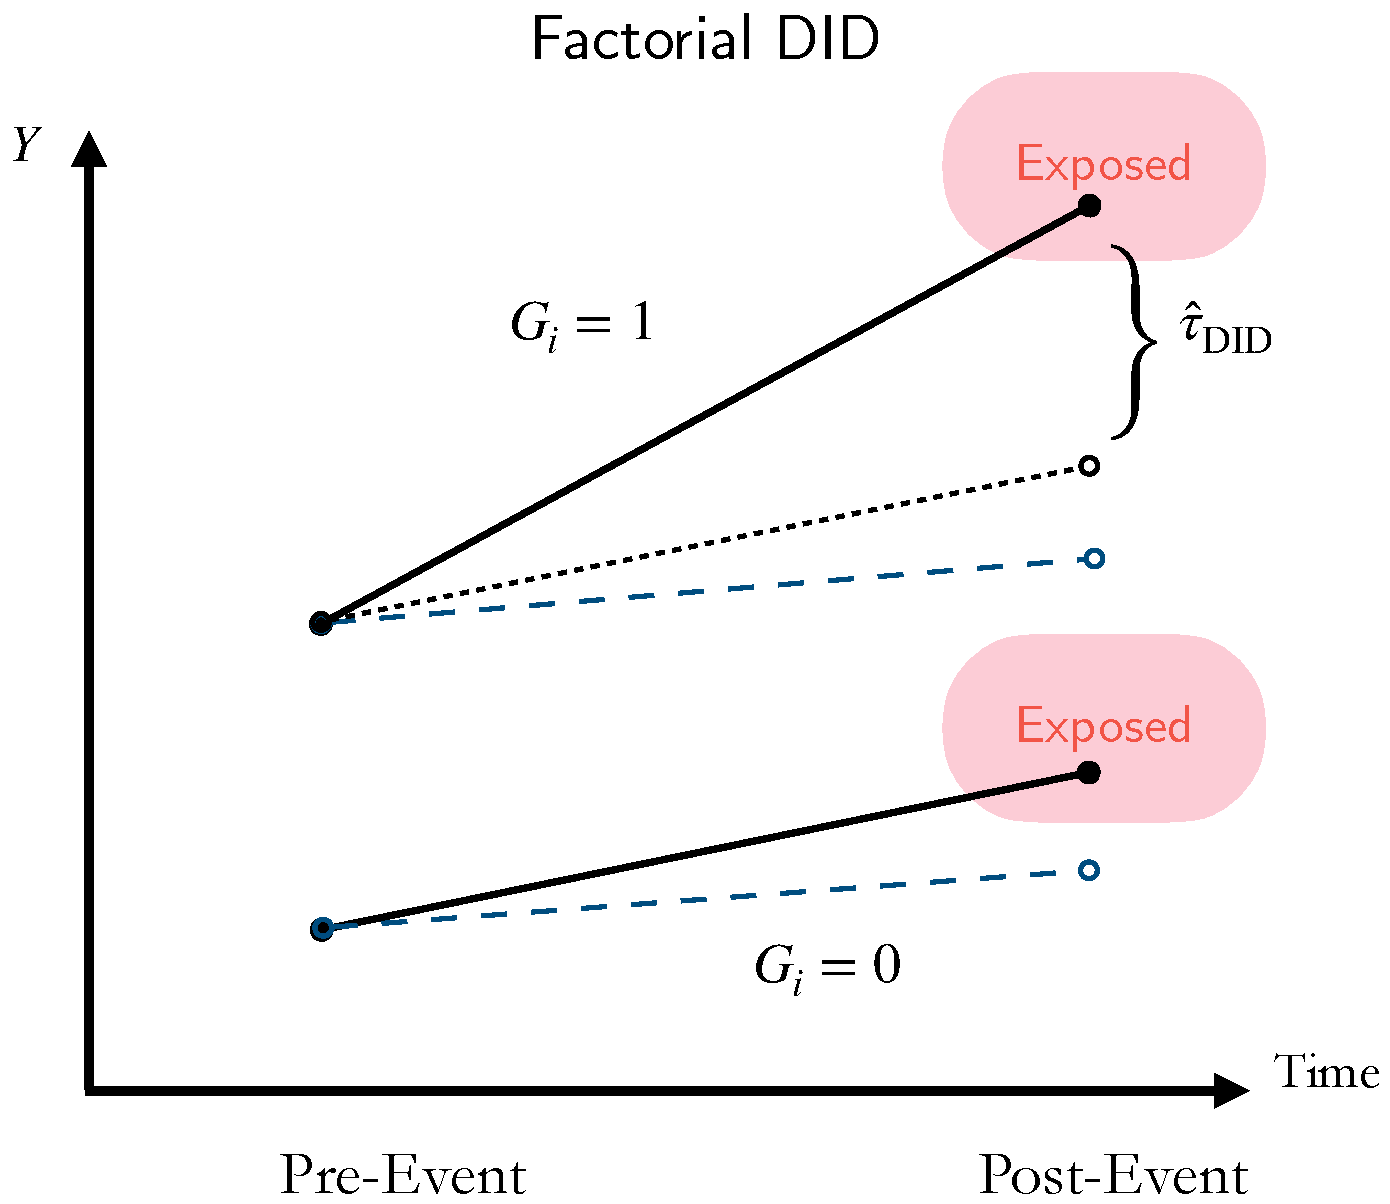
\includegraphics[width=\linewidth, height=0.6\textheight, keepaspectratio]{c_factorial_did.pdf}}
\end{column}
\end{columns}
\end{frame}

\section{Setup and Estimands}

\begin{frame}
  \frametitle{Setup}
\alert{Two groups, two periods; no covariates}
\begin{columns}[T,onlytextwidth]
\begin{column}{0.55\textwidth}
\begin{itemize}[<+->]\itemsep0.7em
\item Study population: $i = 1, 2, \cdots, n$
\item Timing of the event is fixed
\item Time periods: $t=$ pre, post
\item Baseline factor: $G_i \in \{0,1\}$
\item Data: $\{G_i, Y_{i,\pre}, Y_{i,\post}: i = 1, 2, \cdots, n\}$
\item \alert{Universal exposure} to the event in the post period:
$$Z_i = 1, \quad i = 1, 2, \cdots, n$$
\end{itemize}
\end{column}
\begin{column}{0.42\textwidth}
\centering
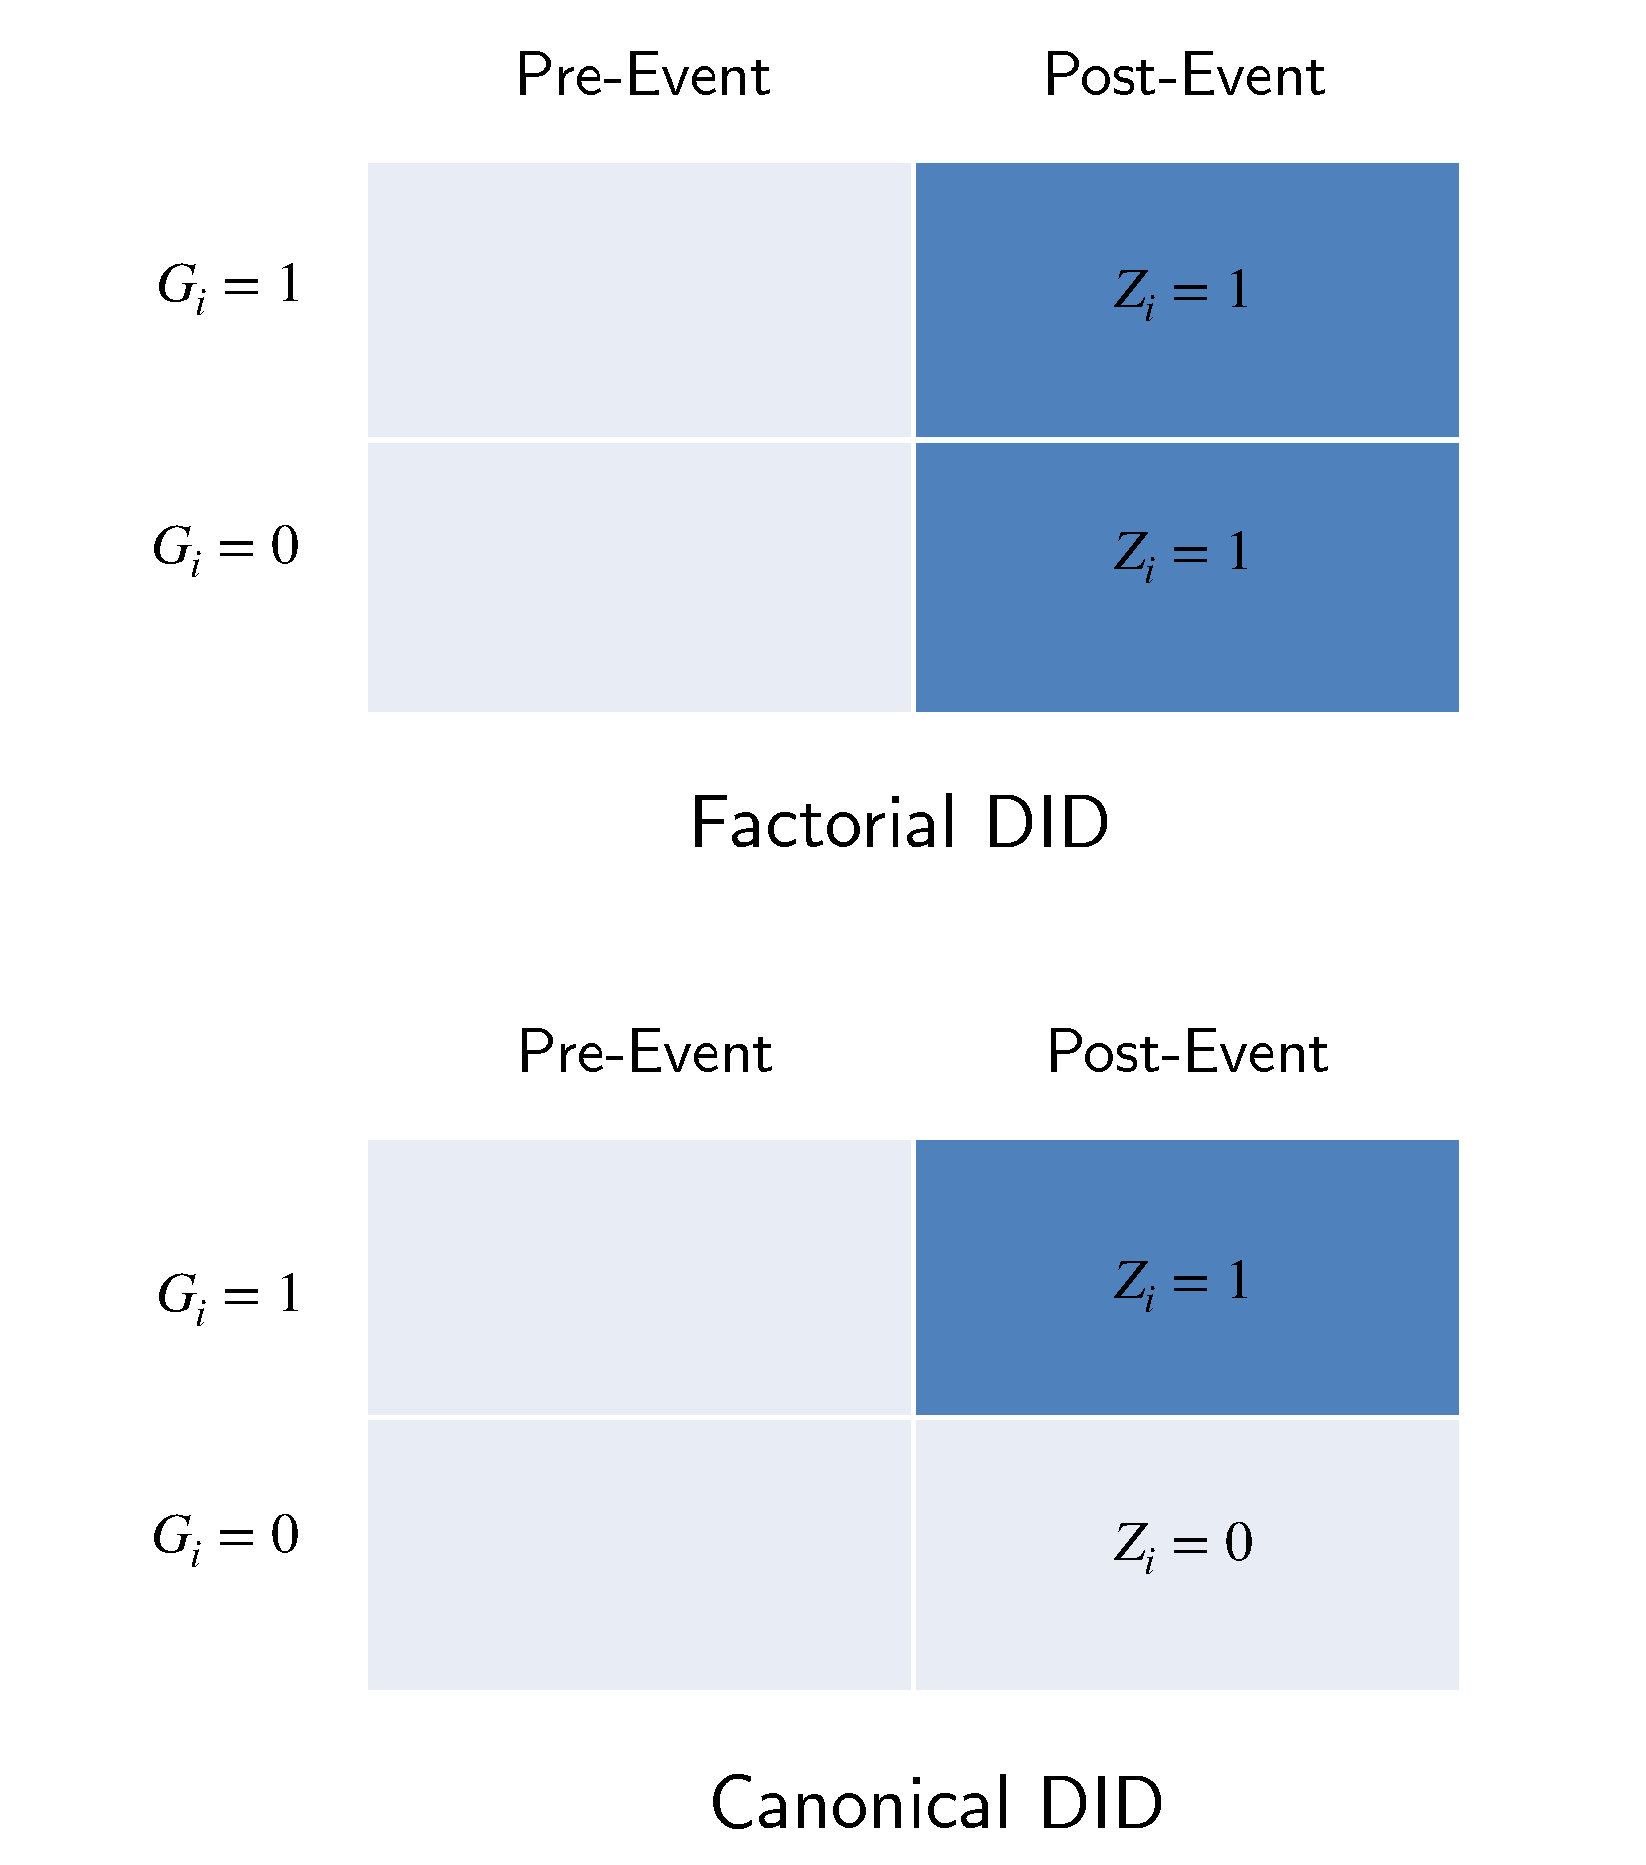
\includegraphics[width=0.9\linewidth, height=0.72\textheight, keepaspectratio]{c_setup_grids.pdf}
\end{column}
\end{columns}
\end{frame}

\begin{frame}
  \frametitle{The Difference-in-Differences Estimator}
\begin{center}
\renewcommand{\arraystretch}{2.1}
\begin{tabular}{c|cc}
 & \textbf{Pre-Event} & \textbf{Post-Event} \\ \hline
$G_i = 1$ & $\dfrac{1}{n_1}\displaystyle\sum_{i: G_i=1} Y_{i,\pre}$ & $\dfrac{1}{n_1}\displaystyle\sum_{i: G_i=1} Y_{i,\post}$ \\
$G_i = 0$ & $\dfrac{1}{n_0}\displaystyle\sum_{i: G_i=0} Y_{i,\pre}$ & $\dfrac{1}{n_0}\displaystyle\sum_{i: G_i=0} Y_{i,\post}$ \\
\end{tabular}
\end{center}
\bigskip\pause
Define
\begin{itemize}\itemsep0.7em
\item $\tdidhat = \dfrac{1}{n_1}\displaystyle\sum_{i: G_i=1}\left(Y_{i,\post} - Y_{i,\pre}\right) - \dfrac{1}{n_0}\displaystyle\sum_{i: G_i=0}\left(Y_{i,\post} - Y_{i,\pre}\right)$\pause
\item Focus on: $\text{plim }\tdidhat = \red{\tdid} = \E[\Delta Y_i \mid G_i = 1] - \E[\Delta Y_i \mid G_i = 0]$
\end{itemize}
\end{frame}

\begin{frame}
  \frametitle{Potential Outcomes}
\begin{columns}[T,onlytextwidth]
\begin{column}{0.5\textwidth}
\begin{itemize}[<+->]\itemsep0.9em
\item Frame factorial DID as a factorial design with two factors: $g$ and $z$
\item Potential outcomes indexed by both: $Y_{i,t}(g,z)$
\item Observed outcomes:
$$Y_{i,t} = \sum_{g,z \in \{0,1\}} \mathbf{1}\{G_i = g, Z_i = z\} \cdot Y_{i,t}(g,z) = Y_{i,t}(G_i, Z_i)$$
\item Recall: in observed data, $Z_i = 1$ for all units
$\Rightarrow$ \red{half of the potential outcomes are never observed}
\end{itemize}
\end{column}
\begin{column}{0.47\textwidth}
\centering
\onslide<2->{\resizebox{\linewidth}{!}{\potree{0}}
\par\smallskip{\scriptsize \red{Red}: potential outcomes never observed under universal exposure.}}
\end{column}
\end{columns}
\end{frame}

\begin{frame}
  \frametitle{Causal Quantities: Individual Level}
\begin{columns}[T,onlytextwidth]
\begin{column}{0.44\textwidth}
\begin{itemize}[<+->]\itemsep1em
\item Individual conditional effect of the event at factor level $g$:
$$\tau_{i,Z|G=g} = Y_{i,\post}(g,1) - \red{Y_{i,\post}(g,0)}$$
\item Individual interaction effect:
\begin{align*}
\tau_{i,\mathrm{cm}} &= Y_{i,\post}(1,1) - \red{Y_{i,\post}(1,0)}\\
&\quad - Y_{i,\post}(0,1) + \red{Y_{i,\post}(0,0)}\\
&= \tau_{i,Z|G=1} - \tau_{i,Z|G=0}
\end{align*}
the \alert{causal moderation} of $G$ on $Z$
\end{itemize}
\end{column}
\begin{column}{0.53\textwidth}
\centering
\resizebox{\linewidth}{!}{\potree{1}}
\end{column}
\end{columns}
\end{frame}

\begin{frame}
  \frametitle{Causal Quantities: Averages}
\begin{itemize}\itemsep0.6em
\item \textbf{Average causal interaction} {\small\parencite{vanderweele2009distinction,bansak2021estimating}}:
$$\tcm = \E[Y_{i,\post}(1,1) - Y_{i,\post}(1,0) - Y_{i,\post}(0,1) + Y_{i,\post}(0,0)] = \E[\tau_{i,Z|G=1}] - \E[\tau_{i,Z|G=0}]$$
\end{itemize}
\begin{block}{}
\centering ``Social capital \underline{reduced} the mortality increase caused by the famine.''
\end{block}
\medskip\pause
\begin{itemize}\itemsep0.6em
\item \textbf{Effect modification} --- associative:
$$\tem = \E[\tau_{i,Z|G=1} \mid G_i = 1] - \E[\tau_{i,Z|G=0} \mid G_i = 0]$$
\end{itemize}
\begin{block}{}
\centering ``Places with higher social capital \underline{experienced} a smaller mortality increase caused by the famine.''
\end{block}
\medskip\pause
\begin{itemize}
\item The verbs differ because the estimands differ: \tcm{} is causal, \tem{} compares \alert{different units}
\end{itemize}
\end{frame}

\section{Identification}

\begin{frame}
  \frametitle{Identification: A Roadmap}
\begin{center}
\idmap{0}
\end{center}
\end{frame}

\begin{frame}
  \frametitle{Identification under Canonical DID Assumptions}
\begin{columns}[T,onlytextwidth]
\begin{column}{0.46\textwidth}
\begin{block}{No Anticipation}
$Y_{i,\red{\pre}}(g,0) = Y_{i,\red{\pre}}(g,1)$ for all $i$ and $g = 0,1$
\end{block}
\medskip
\begin{block}{Parallel Trends}
$\E[\red{\Delta Y_i(1,0)} \mid G_i = 1] = \E[\red{\Delta Y_i(0,0)} \mid G_i = 0]$
\end{block}
\medskip
\onslide<2->{%
\begin{block}{Proposition}
Under no anticipation and parallel trends,
{\small$$\tdid = \tem = \E[\tau_{i,Z|G=1} \mid G_i = 1] - \E[\tau_{i,Z|G=0} \mid G_i = 0]$$}
\end{block}
\smallskip
{\small Two different \red{conditional effects}, across two different \textcolor{SlideInk}{groups}}}
\end{column}
\begin{column}{0.51\textwidth}
\centering
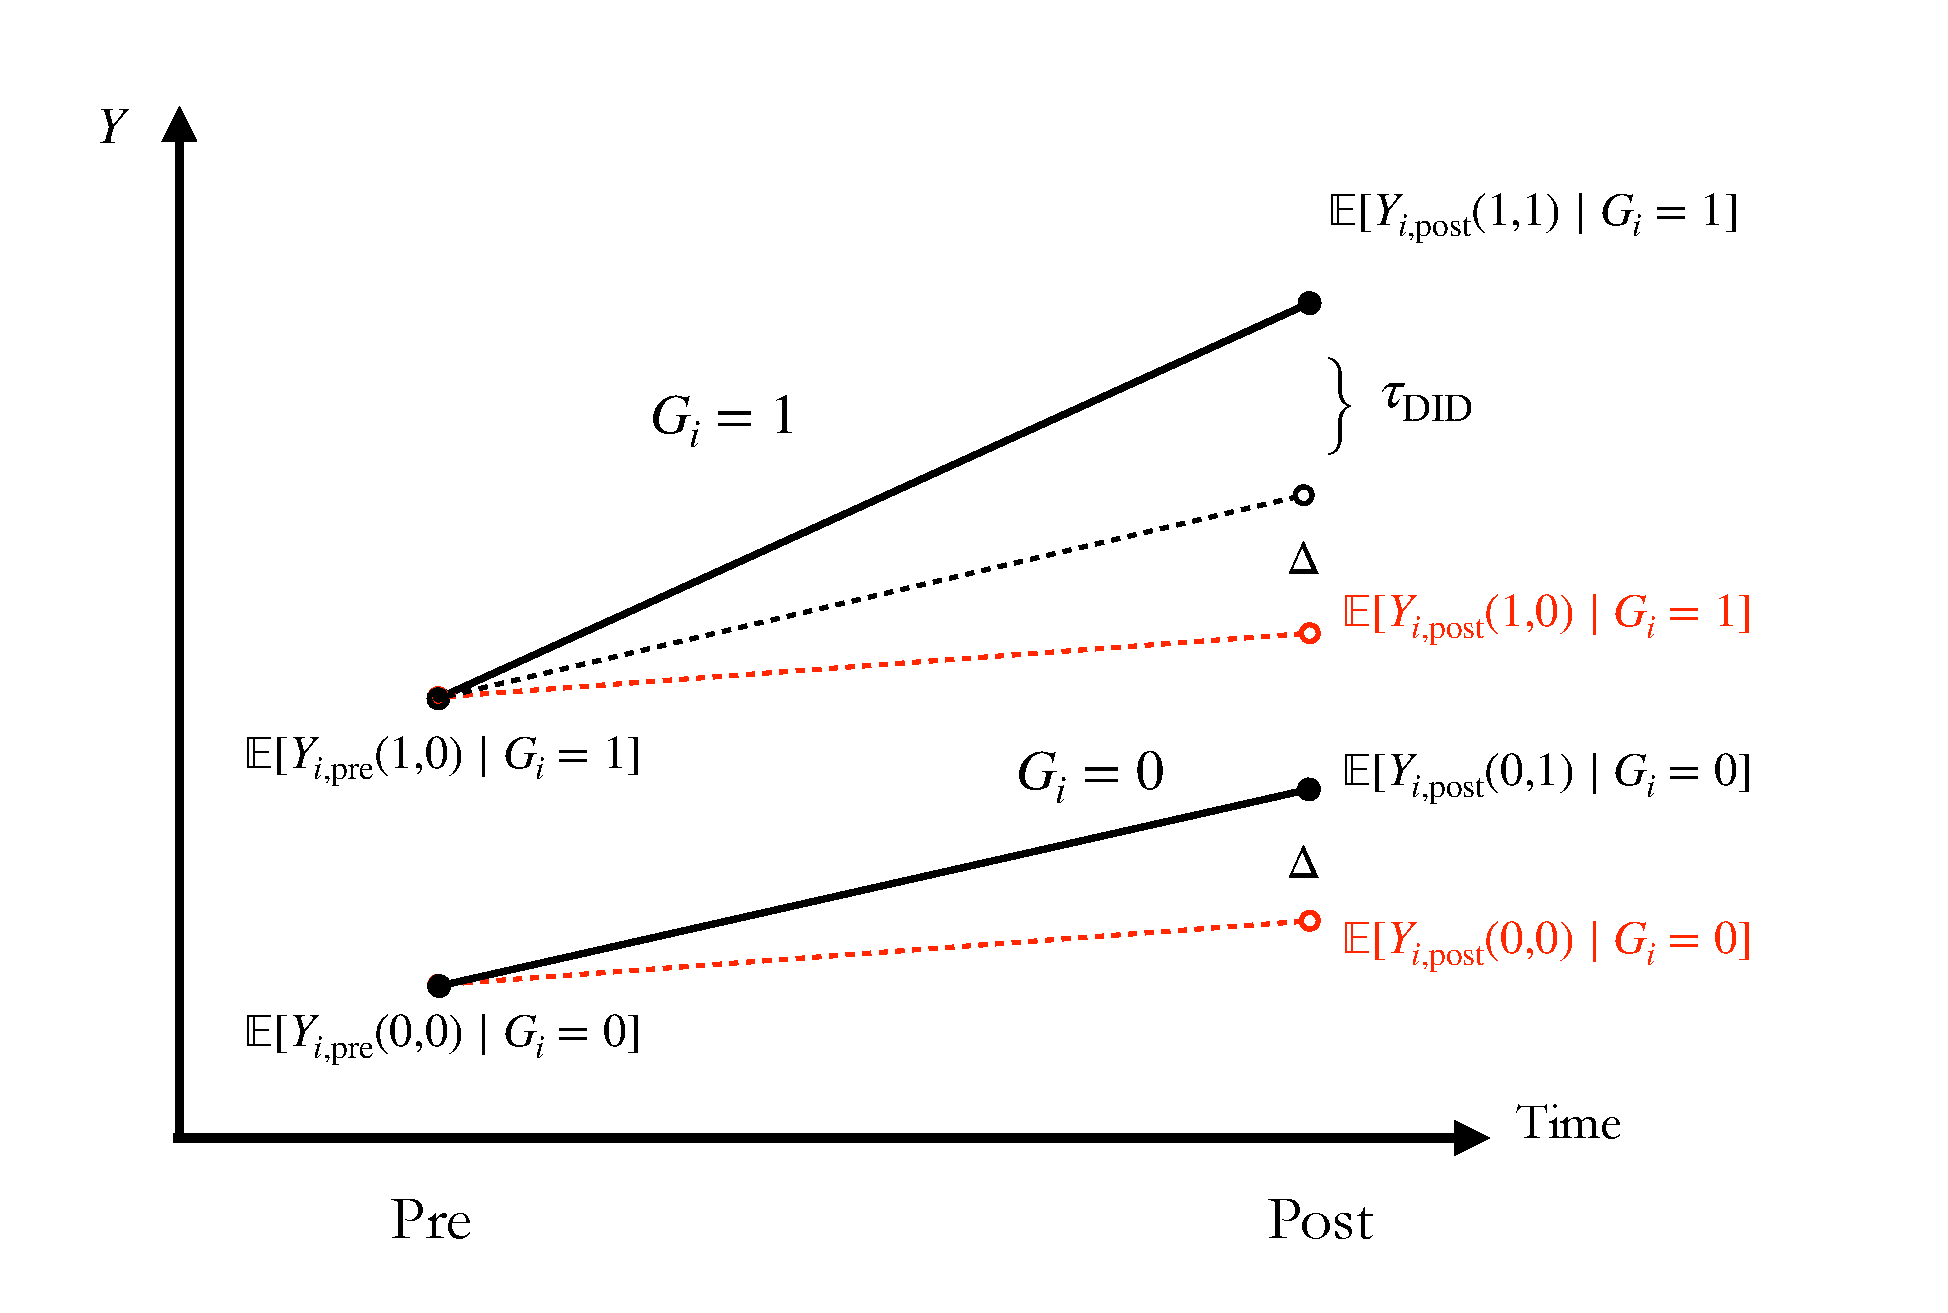
\includegraphics[width=\linewidth]{c_canonical_graph.pdf}
\end{column}
\end{columns}
\end{frame}

\begin{frame}[t]
  \frametitle{Why $\tdid$ May Not Identify Causal Moderation under Parallel Trends}
\begin{columns}[T,onlytextwidth]
\begin{column}{0.46\textwidth}
\centering
\only<1-2| handout:0>{\twogroupfig{Both groups: $U = 1/4$}{$G_i = 1,\ U_i = 1/4$}{$G_i = 0,\ U_i = 1/4$}{0.5}{0.5}{$\tdid = 0$}{f}}%
\only<3| handout:0>{\twogroupfig{Both groups: $U = 3/4$}{$G_i = 1,\ U_i = 3/4$}{$G_i = 0,\ U_i = 3/4$}{1.5}{1.5}{$\tdid = 0$}{f}}%
\only<4| handout:0>{\twogroupfig{$U$ differs across groups}{$G_i = 1,\ U_i = 3/4$}{$G_i = 0,\ U_i = 1/4$}{1.5}{0.5}{}{f}}%
\only<5-| handout:1>{\twogroupfig{$U$ differs across groups}{$G_i = 1,\ U_i = 3/4$}{$G_i = 0,\ U_i = 1/4$}{1.5}{0.5}{$\tdid = \tem$}{f}}
\end{column}
\begin{column}{0.5\textwidth}
\begin{itemize}\itemsep1em
\item Imagine an unobservable $U$ that determines how units respond to the event
\begin{itemize}\itemsep0.3em
  \item<2-> If both groups share the same $U$, the event moves them equally and $\tdid = 0$, whether $U$ is small or large
\end{itemize}
\item<4-> $U$ may be \alert{correlated with $G$}: here, high-$U$ units ($U_i = 3/4$) are concentrated in $G=1$
\item<5-> Then $\tdid = \tem$ mixes the moderation of $G$ with \alert{compositional differences} in $U$
\item<6-> Therefore $\tdid$ cannot be interpreted as the causal moderation of $G$
\end{itemize}
\end{column}
\end{columns}
\end{frame}

\begin{frame}
  \frametitle{Identifying Causal Moderation}
\begin{itemize}\itemsep0.8em
\item Under no anticipation and parallel trends:
$$\tdid = \tem = \E[Y_{i,\post}(1,1) - Y_{i,\post}(1,0) \mid G_i = 1] - \E[Y_{i,\post}(0,1) - Y_{i,\post}(0,0) \mid G_i = 0]$$
\item<2-> When does $\tem$ equal $\tcm$, which drops the conditioning on $G_i$?
\end{itemize}
\medskip
\onslide<3->{%
\begin{block}{Factorial Parallel Trends (sufficient condition)}
$$\red{\Delta Y_i(g,z) \indep G_i} \qquad \text{(orthogonality between $G$ and first-differenced potential outcomes)}$$
\end{block}}
\medskip
\begin{itemize}
\item<4-> Weaker than (quasi-)random assignment of $G$: $Y_{i,t}(g,z) \indep G_i$
\item<5-> Under no anticipation, parallel trends, and $\Delta Y_i(g,z) \indep G_i$: \quad $\tdid = \tem = \tcm$
\end{itemize}
\end{frame}


\begin{frame}[t]
  \frametitle{Reconciling Canonical and Factorial DID}
\begin{columns}[T,onlytextwidth]
\begin{column}{0.46\textwidth}
\centering
\only<1| handout:0>{\twogroupfig{Factorial DID}{$G_i = 1$}{$G_i = 0$}{1.5}{0.5}{$\tdid = \tem$}{f}}%
\only<2| handout:0>{\twogroupfig{Factorial DID}{$G_i = 1$}{$G_i = 0$}{1.5}{0}{$\tdid = \tem$}{z}}%
\only<3-| handout:1>{\twogroupfig{Factorial DID $\rightarrow$ Canonical DID}{$G_i = 1$}{$G_i = 0$}{1.5}{0}{$\tdid = \tatt$}{c}}
\end{column}
\begin{column}{0.5\textwidth}
\onslide<2->{%
\begin{block}{Exclusion Restriction on $Z$ for Group $G_i=0$}
$$\E[Y_{i,\post}(0,1) \mid G_i = 0] = \E[Y_{i,\post}(0,0) \mid G_i = 0]$$
the event does not move $G=0$ units: their $\Delta$ is zero
\end{block}}
\medskip
\onslide<3->{%
\begin{block}{Proposition}
Under no anticipation, parallel trends, and the exclusion restriction,
$$\tdid = \tatt = \E[Y_{i,\post}(1,1) - Y_{i,\post}(1,0) \mid G_i = 1]$$
\end{block}}
\medskip
\begin{itemize}
\item<4-> This is exactly the canonical DID of Lecture 2: ``untreated'' units are units for which the event is assumed not to matter
\end{itemize}
\end{column}
\end{columns}
\end{frame}

\begin{frame}
  \frametitle{Identifying $G$'s Conditional Effect}
\begin{itemize}\itemsep0.8em
\item One more question the interaction might answer: the \alert{effect of $G$ itself} during the event
\end{itemize}
\medskip
\onslide<2->{%
\begin{block}{Exclusion Restriction on $G$ Absent the Event}
$$\E[Y_{i,\post}(1,0)] = \E[Y_{i,\post}(0,0)]$$
without the event, the baseline factor would not move the outcome
\end{block}}
\medskip
\begin{itemize}\itemsep0.8em
\item<3-> Under no anticipation, parallel trends, factorial parallel trends, and this exclusion restriction:
$$\tdid = \tcm = \E[Y_{i,\post}(1,1) - Y_{i,\post}(0,1)] = \tgz$$
\item<4-> In the famine example: the average causal effect of social capital on mortality \alert{during the famine years}
\end{itemize}
\end{frame}

\begin{frame}
  \frametitle{Summary of Identification Results}
\begin{center}
\idmap{1}
\end{center}
\end{frame}

\begin{frame}
  \frametitle{Canonical vs Factorial DID: Two Research Designs}
\begin{block}{Canonical DID (reframed)}
Define the \underline{canonical DID research design} as the combination of:
\begin{itemize}\itemsep0.3em
\item $2\times 2$ data structure \& \alert{universal exposure}
\item Identification: under no anticipation \& parallel trends \& \red{exclusion restriction on $Z$}, $\tdidhat$ identifies \tatt
\end{itemize}
\end{block}
\medskip\pause
\begin{block}{Factorial DID}
Define the \underline{factorial DID research design} as the combination of:
\begin{itemize}\itemsep0.3em
\item $2\times 2$ data structure \& \alert{universal exposure}
\item Identification:
\begin{enumerate}\itemsep0.25em
\item Under no anticipation \& parallel trends, $\tdidhat$ identifies \tem
\item Adding $\red{\Delta Y_i(g,z) \indep G_i}$, $\tdidhat$ identifies \tcm
\item Adding also the \red{exclusion restriction on $G$}, $\tdidhat$ identifies \tgz
\end{enumerate}
\end{itemize}
\end{block}
\end{frame}

\section{Extensions}

\begin{frame}
  \frametitle{Conditioning on Covariates in Practice}
\begin{itemize}
\item Researchers often run the following TWFE regression:
$$Y_{it} = \alpha_i + \xi_t + \red{\tau}\, G_i\cdot\mathrm{Post}_t + \beta^{\mathrm{T}}\textcolor{SlideInk}{X_i\cdot\mathrm{Post}_t} + \epsilon_{it}$$
\end{itemize}
\begin{center}
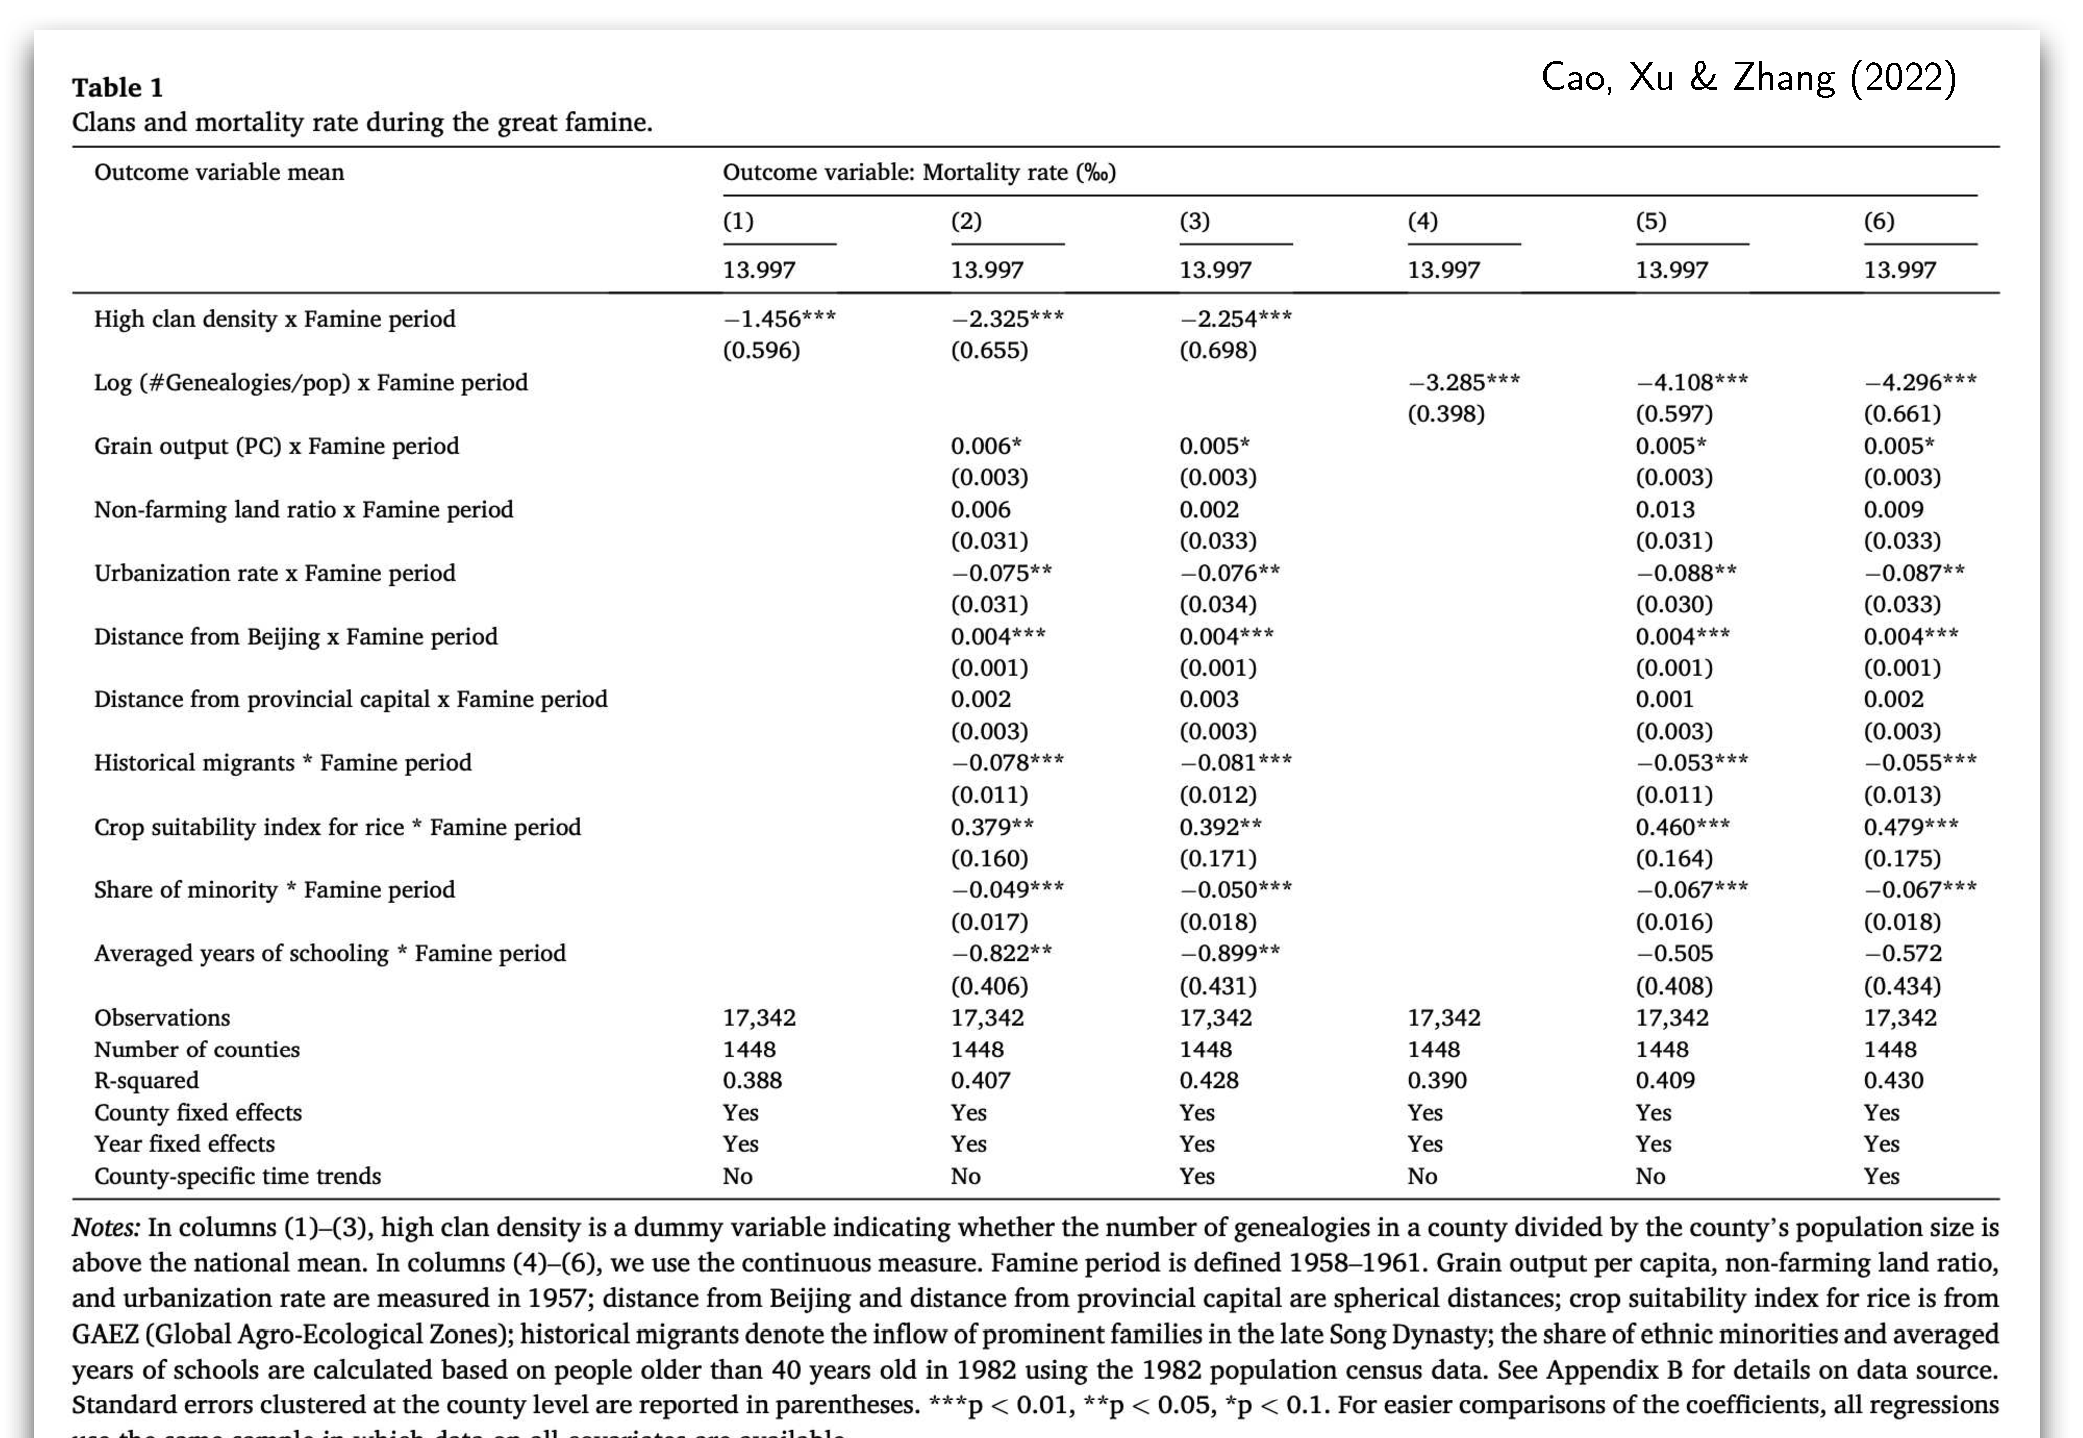
\includegraphics[width=0.62\textwidth, height=0.58\textheight, keepaspectratio]{c_cxz_table.pdf}
\end{center}
\end{frame}

\begin{frame}
  \frametitle{Extension to Conditionally Valid Assumptions}
\begin{itemize}[<+->]\itemsep0.8em
\item Believe $\Delta Y_i(g,z) \indep G_i \mid X_i$ is more plausible than $\Delta Y_i(g,z) \indep G_i$
\item Simple improvements to the TWFE regression: (a) demean $X_i$; (b) add interaction terms
$$Y_{it} = \alpha_i + \xi_t + \red{\tau}\, G_i\cdot\mathrm{Post}_t + \beta^{\mathrm{T}} X_i\cdot\mathrm{Post}_t + \gamma^{\mathrm{T}}\red{G_i\cdot X_i\cdot\mathrm{Post}_t} + \epsilon_{it}$$
\begin{itemize}\itemsep0.4em
  \item $\hat{\tau}$ identifies $\E[\tem(x)]$, or \tcm{} under linearity
  \item Requires overlap: $0 < \mathbb{P}(G_i = 1 \mid X_i = x) < 1$
\end{itemize}
\item Can leverage more flexible models of $\Delta Y_i$ on $X_i$ for subgroups $G_i = 1, 0$:
\begin{itemize}\itemsep0.4em
  \item Transform data into wide form; replace $Y_i$ with $\Delta Y_i$
  \item Apply estimators developed for selection-on-observables designs\\
  {\small (stratification, matching, balancing, IPW, AIPW, outcome modeling, double machine learning, \ldots)}
\end{itemize}
\end{itemize}
\end{frame}

\begin{frame}
  \frametitle{Extension to Multiple Pre- and Post-Periods}
\begin{center}
\begin{tikzpicture}
\node[anchor=south west, inner sep=0] (img) {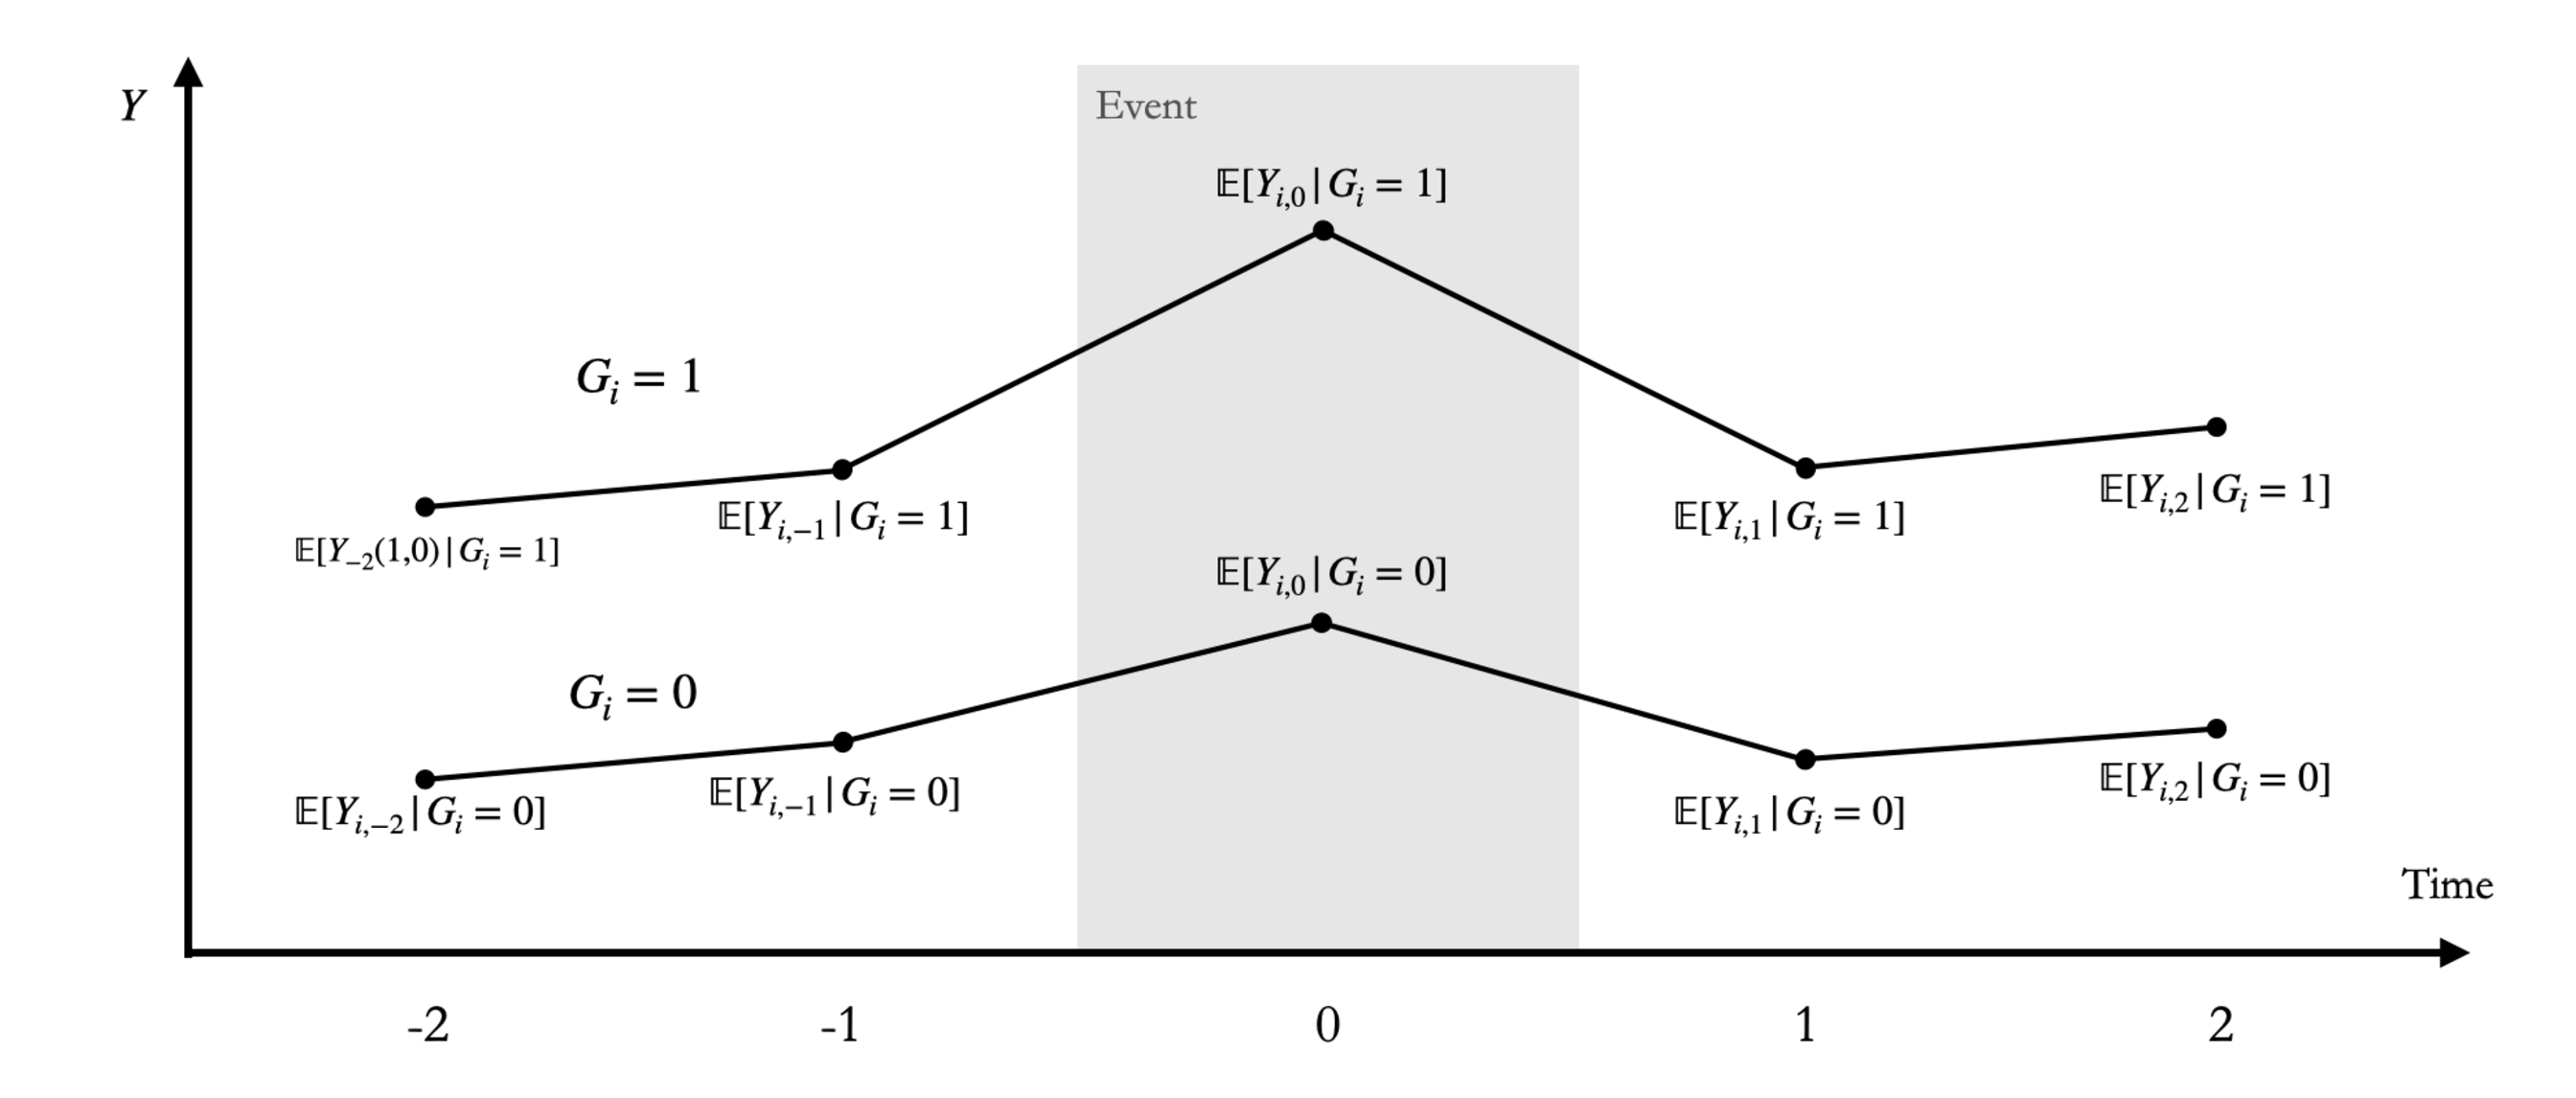
\includegraphics[width=0.72\textwidth, height=0.58\textheight, keepaspectratio]{c_multiperiod.pdf}};
\begin{scope}[x={(img.south east)},y={(img.north west)}]
\fill[white] (0.0,0.40) rectangle (0.165,0.545);
\fill[white] (0.165,0.42) rectangle (0.218,0.51);
\node[font=\tiny] at (0.078,0.445) {$\E[Y_{i,-2} \mid G_i = 1]$};
\end{scope}
\end{tikzpicture}
\end{center}
\begin{itemize}\itemsep0.5em
\item<2-> \underline{Lesson 1}: pretrend tests can help assess parallel trends, but \red{not} $\Delta Y(g,z) \indep G$
\item<3-> \underline{Lesson 2}: using post-periods as non-event periods requires an additional ``no carryover effect'' assumption
\end{itemize}
\end{frame}

\section{Application: Clans and Calamity}

\begin{frame}[t]
  \frametitle{Example: Clans and Calamity}
\begin{columns}[T,onlytextwidth]
\begin{column}{0.42\textwidth}
\begin{itemize}\itemsep0.9em
\item Event: the Great Famine (1958--1961)
\item<2-> $G$: social capital, proxied by genealogy books
\begin{itemize}\itemsep0.4em
  \item<2-> No genealogies: 412 counties
  \item<2-> Have pre-PRC genealogies: 509 counties
\end{itemize}
\item<3-> Outcome: county mortality rate
\end{itemize}
\end{column}
\begin{column}{0.55\textwidth}
\centering
\only<1| handout:0>{%
\begin{tikzpicture}
\node[anchor=south west, inner sep=0] (m) at (0,0) {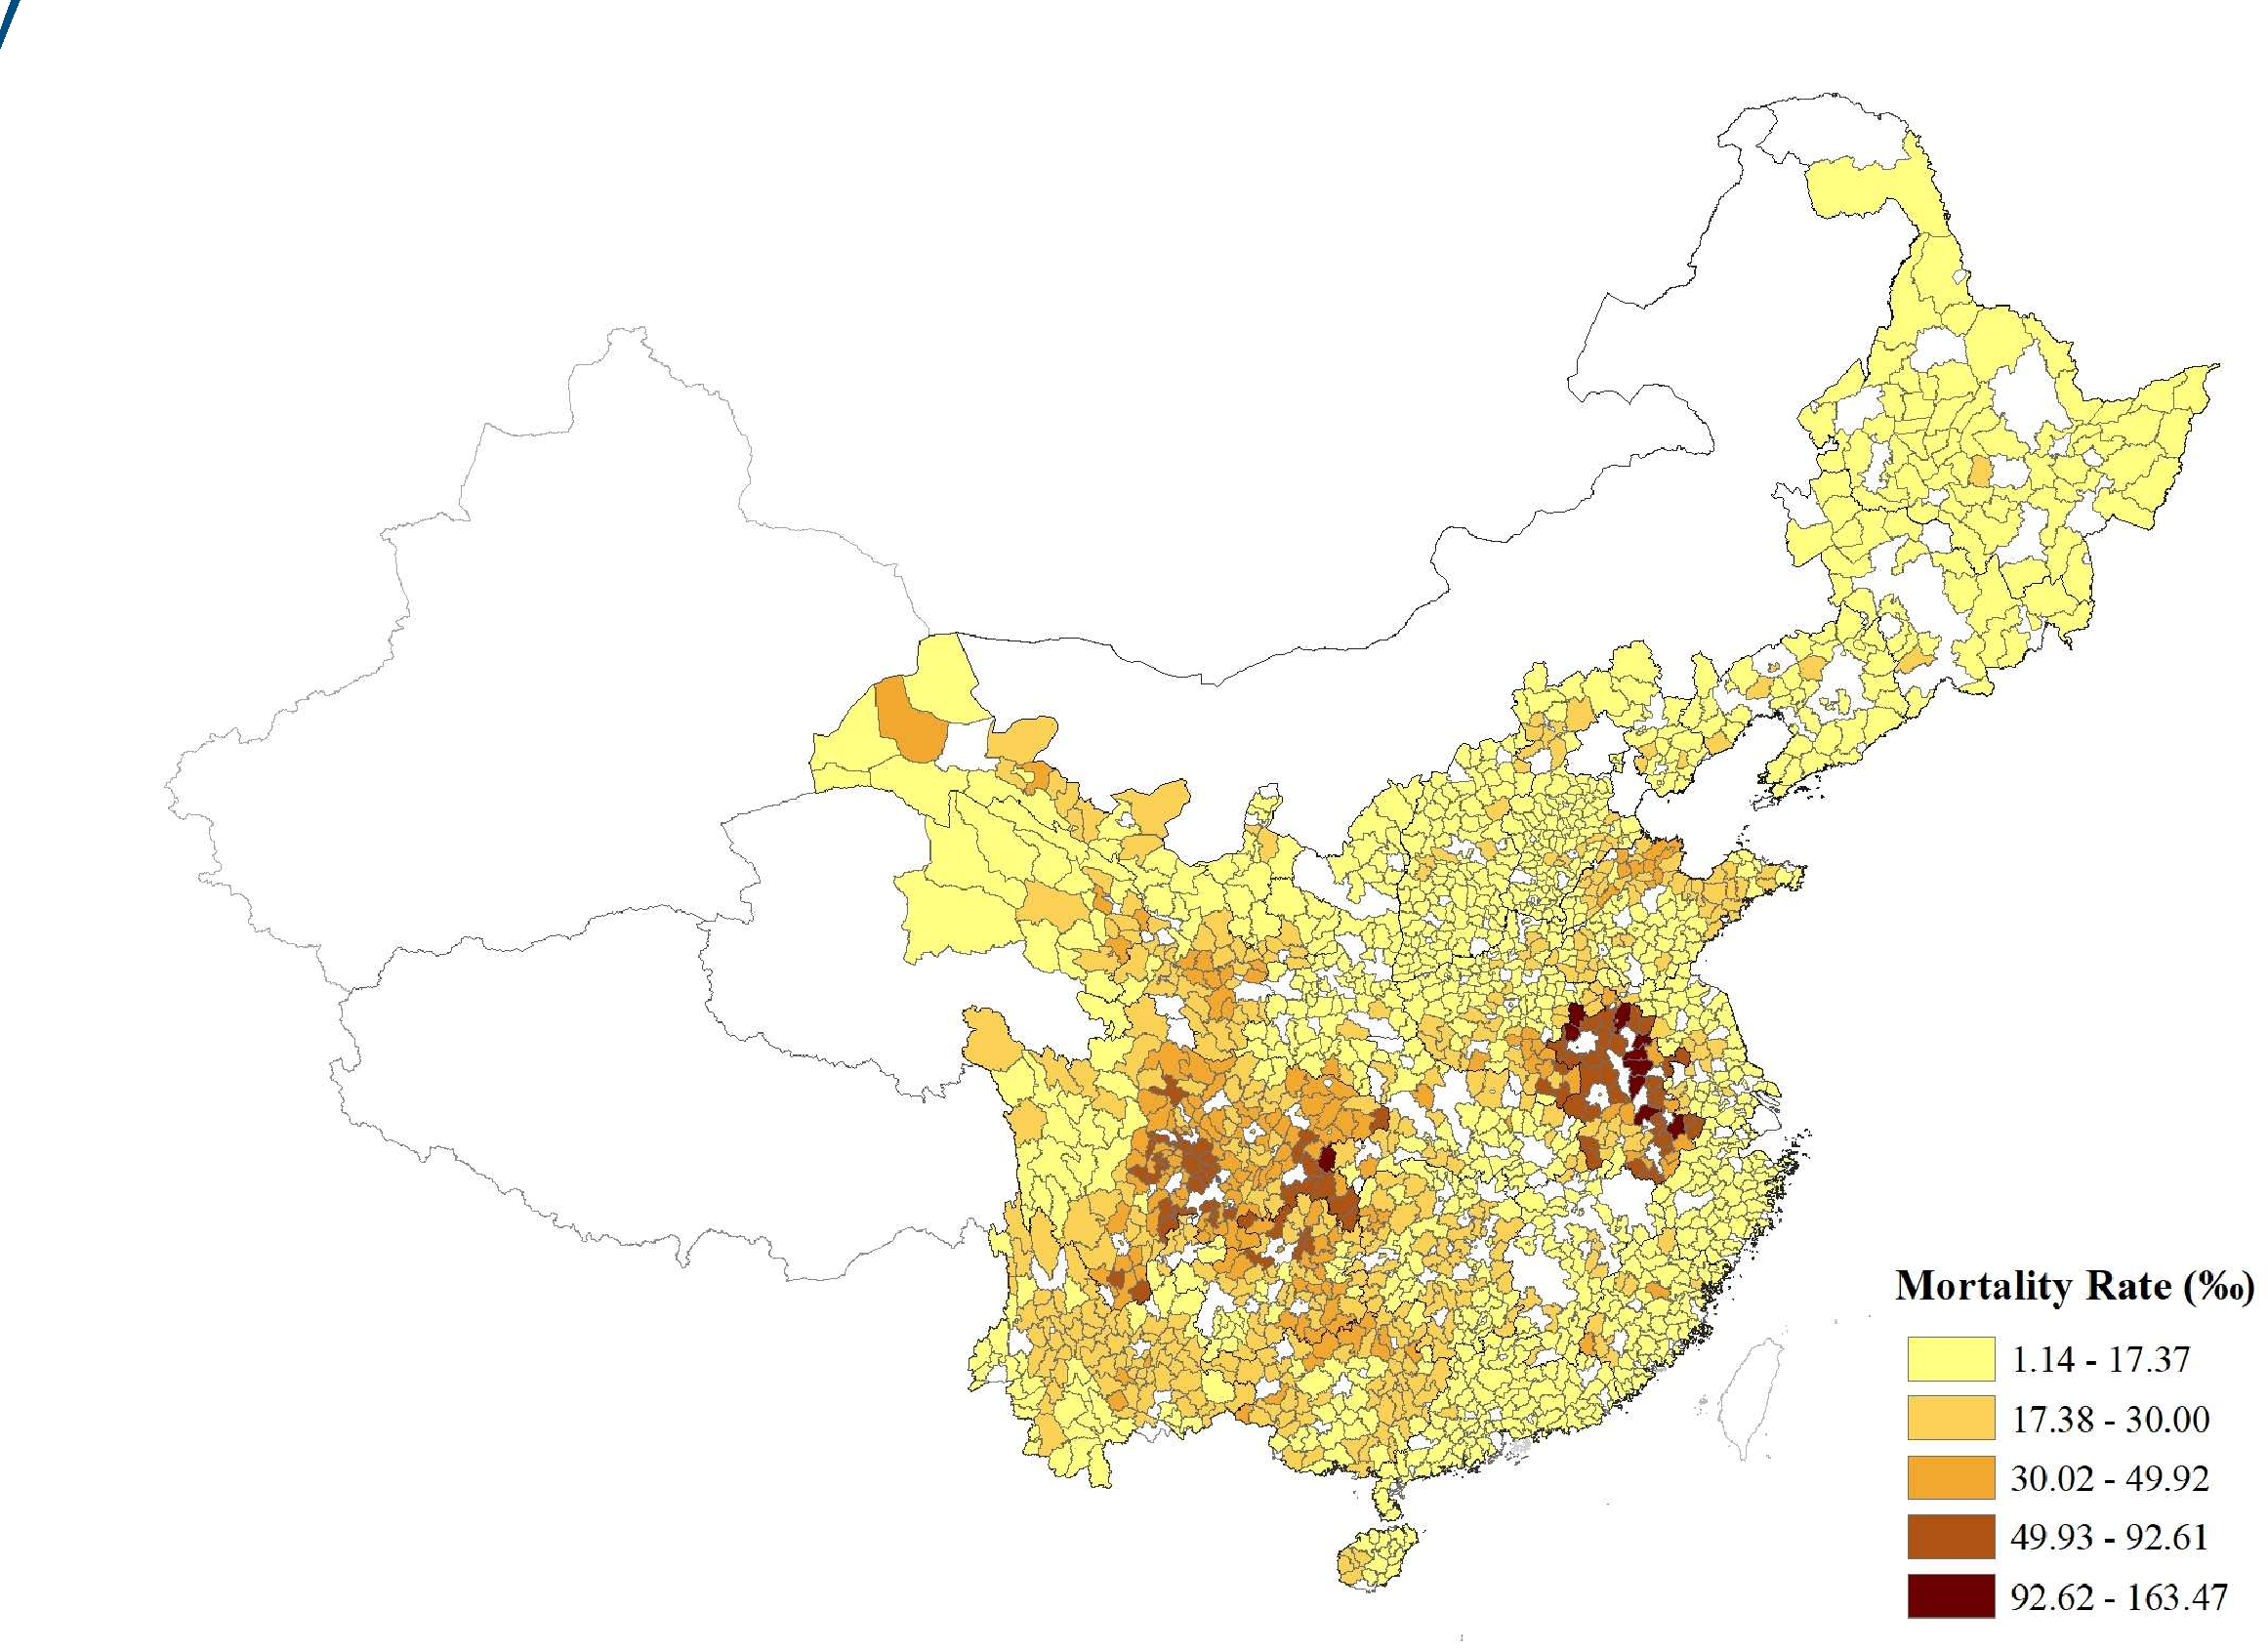
\includegraphics[width=\linewidth, height=0.7\textheight, keepaspectratio]{c_map_mortality.pdf}};
\fill[white, overlay] let \p1=(m.north west), \p2=(m.south east) in ({\x1-0.0100*(\x2-\x1)},{\y1+0.0000*(\y2-\y1)}) rectangle ({\x1+0.0117*(\x2-\x1)},{\y1+0.0320*(\y2-\y1)});
\end{tikzpicture}}%
\only<2-| handout:1>{%
\begin{tikzpicture}
\node[anchor=south west, inner sep=0] (m) at (0,0) {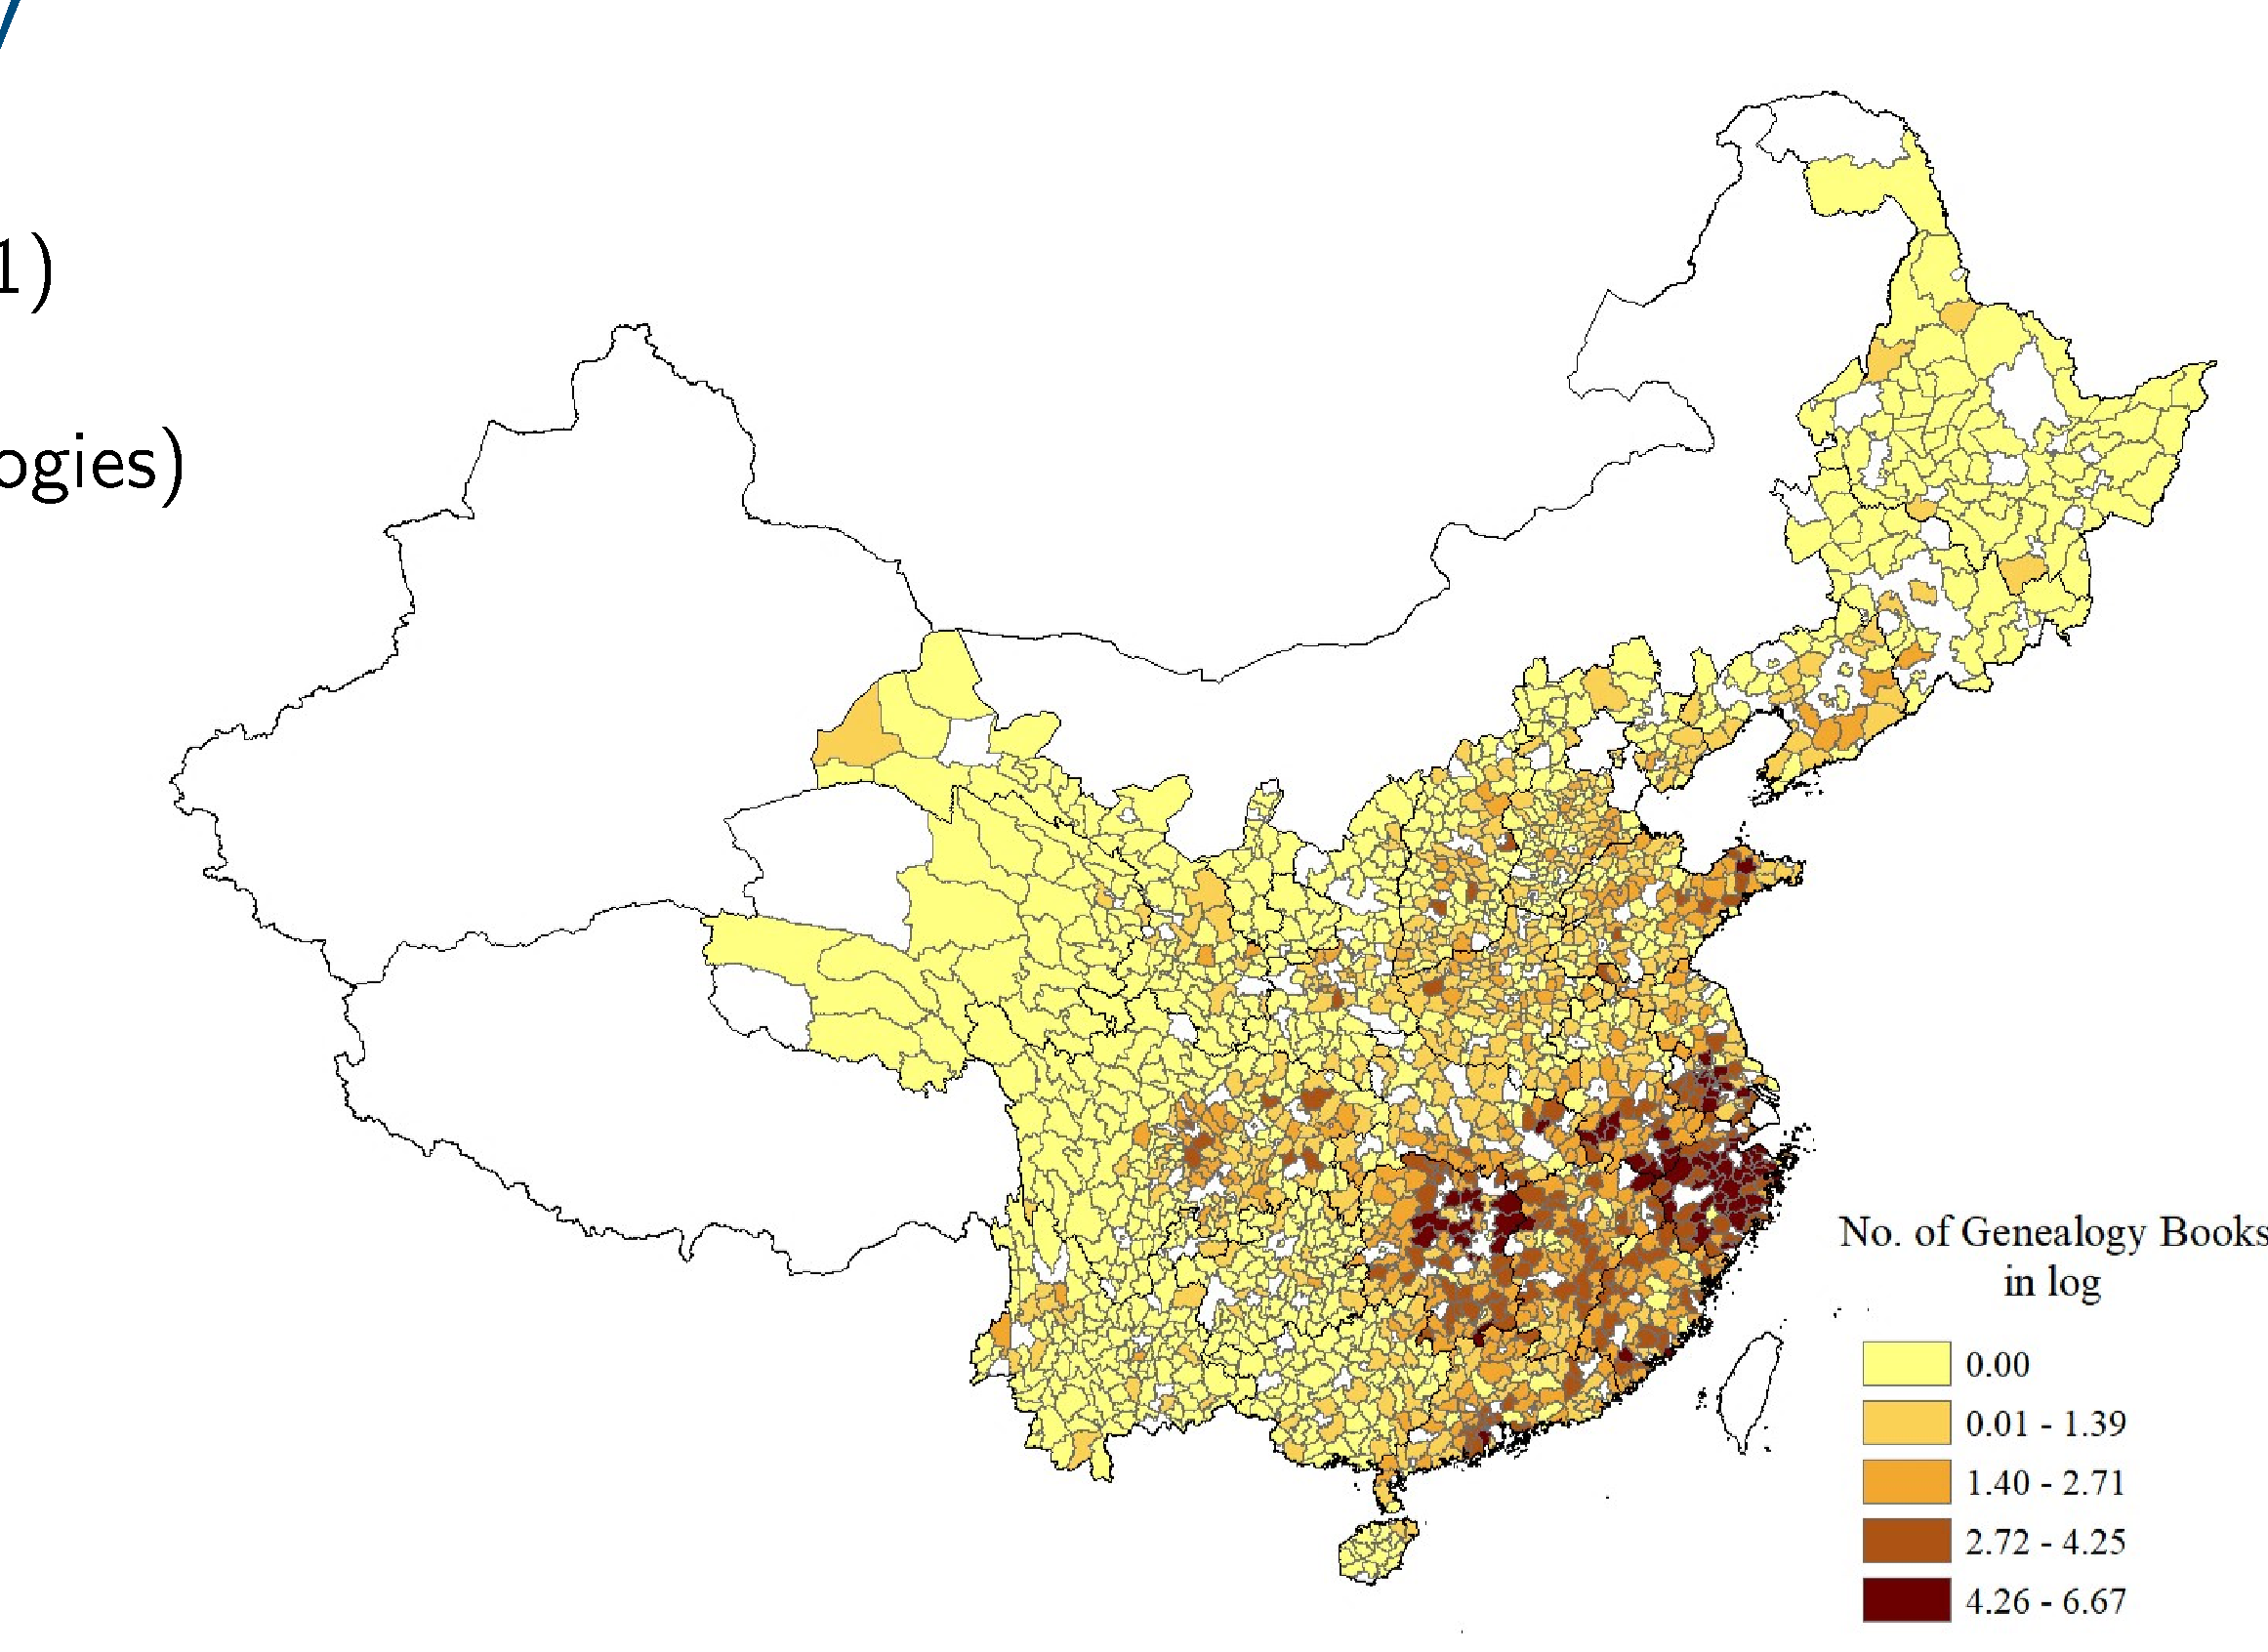
\includegraphics[width=\linewidth, height=0.7\textheight, keepaspectratio]{c_map_genealogy.pdf}};
\begin{scope}
\clip[overlay] let \p1=(m.north west), \p2=(m.south east) in ({\x1-0.0100*(\x2-\x1)},{\y1+0.1281*(\y2-\y1)}) rectangle ({\x1+0.0314*(\x2-\x1)},{\y1+0.1983*(\y2-\y1)}) ({\x1-0.0100*(\x2-\x1)},{\y1+0.2426*(\y2-\y1)}) rectangle ({\x1+0.2278*(\x2-\x1)},{\y1+0.3091*(\y2-\y1)}) ({\x1-0.0100*(\x2-\x1)},{\y1+0.0900*(\y2-\y1)}) rectangle ({\x1+0.0100*(\x2-\x1)},{\y1+0.4200*(\y2-\y1)});
\node[anchor=south west, inner sep=0, overlay] at (-0.3pt,0) {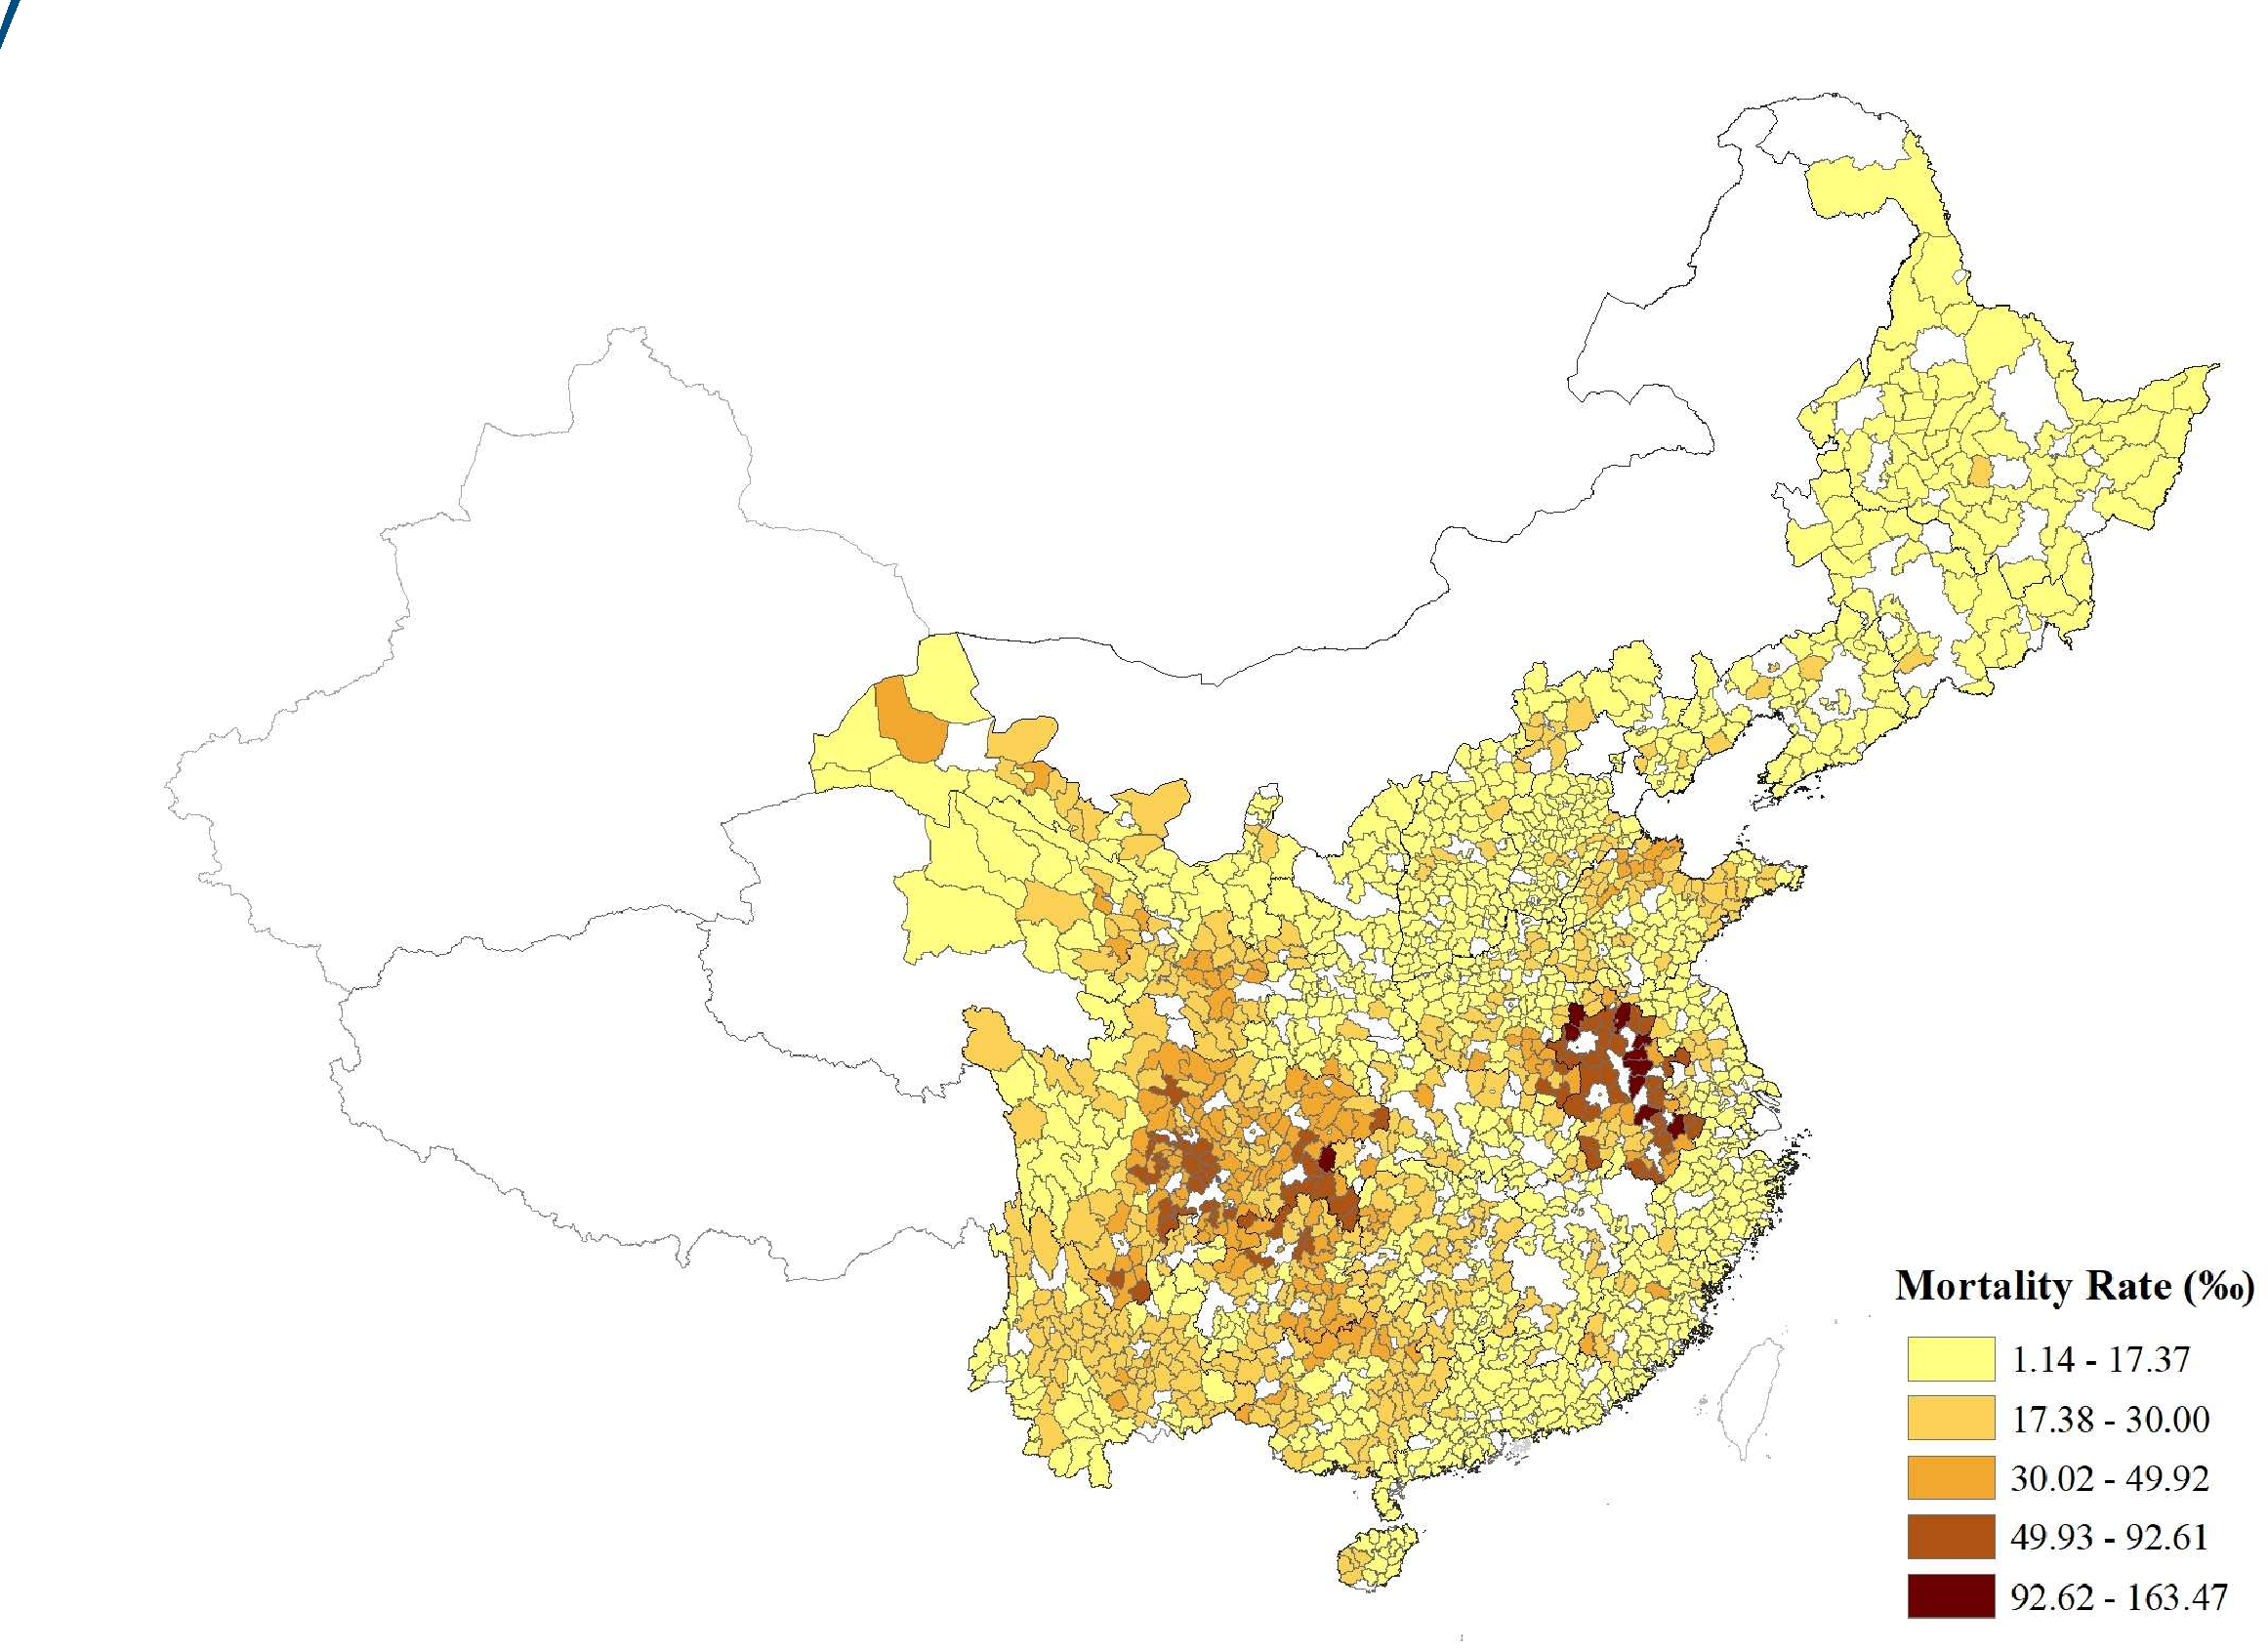
\includegraphics[width=\linewidth, height=0.7\textheight, keepaspectratio]{c_map_mortality.pdf}};
\end{scope}
\fill[white, overlay] let \p1=(m.north west), \p2=(m.south east) in ({\x1-0.0100*(\x2-\x1)},{\y1+0.0000*(\y2-\y1)}) rectangle ({\x1+0.0117*(\x2-\x1)},{\y1+0.0320*(\y2-\y1)});
\end{tikzpicture}}
\end{column}
\end{columns}
\slidesource{\textcite{cao2022clans}; replication data in the \texttt{fdid} R package.}
\end{frame}

\begin{frame}
  \frametitle{Raw Data: Group Means}
\begin{center}
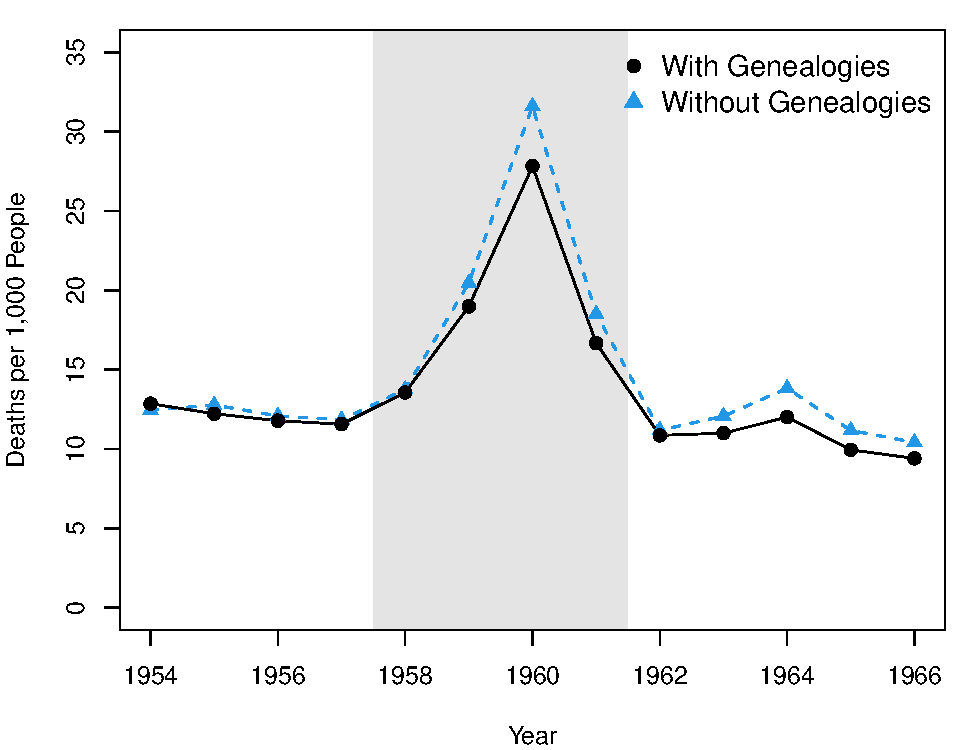
\includegraphics[height=0.78\textheight, keepaspectratio=1]{raw.pdf}
\end{center}
\end{frame}

\begin{frame}
  \frametitle{Conditional on Covariates}
\begin{columns}[T,onlytextwidth]
\begin{column}{0.38\textwidth}
\begin{itemize}\itemsep0.4em
\item Pre-event covariates:
\begin{itemize}\itemsep0.3em
  \item Log population size
  \item Per capita grain production
  \item Ratio of non-farming land
  \item Urbanization ratio
  \item Distance from Beijing
  \item Distance from the provincial capital
  \item Share of ethnic minorities
  \item Rice suitability
  \item Average years of education
\end{itemize}
\end{itemize}
\end{column}
\begin{column}{0.59\textwidth}
\centering
\onslide<2->{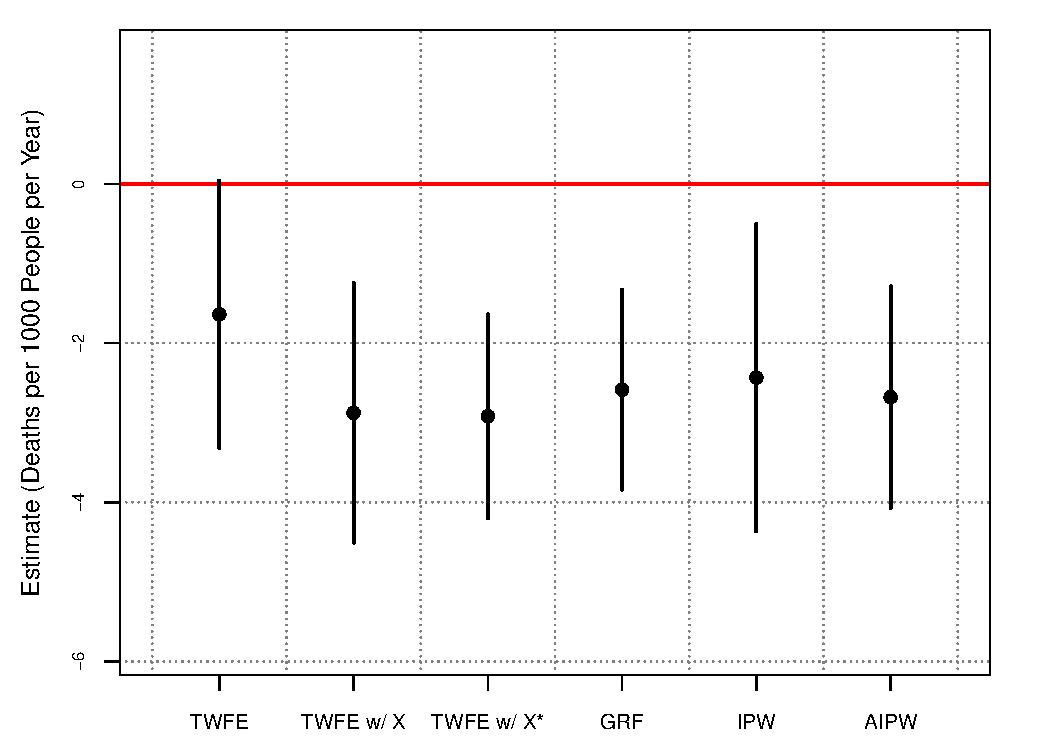
\includegraphics[width=\linewidth, height=0.72\textheight, keepaspectratio]{est_any.pdf}}
\end{column}
\end{columns}
\begin{itemize}
\item<3-> Estimates are stable across estimators, from TWFE to AIPW
\end{itemize}
\end{frame}

\begin{frame}
  \frametitle{Dynamic Estimates: DID}
\begin{center}
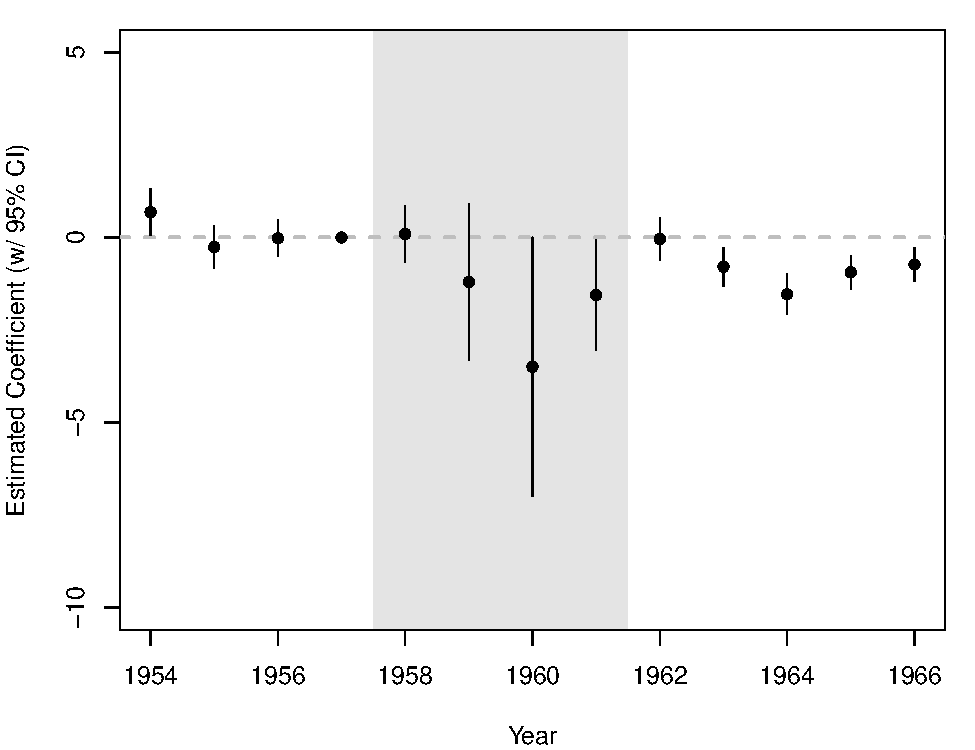
\includegraphics[height=0.78\textheight, keepaspectratio=1]{dyn_did.pdf}
\end{center}
\end{frame}

\begin{frame}
  \frametitle{Dynamic Estimates: TWFE with Covariates}
\begin{columns}[T,onlytextwidth]
\begin{column}{0.49\textwidth}
\centering
{\small TWFE$^{+}$: covariates $\times$ Post}\par\smallskip
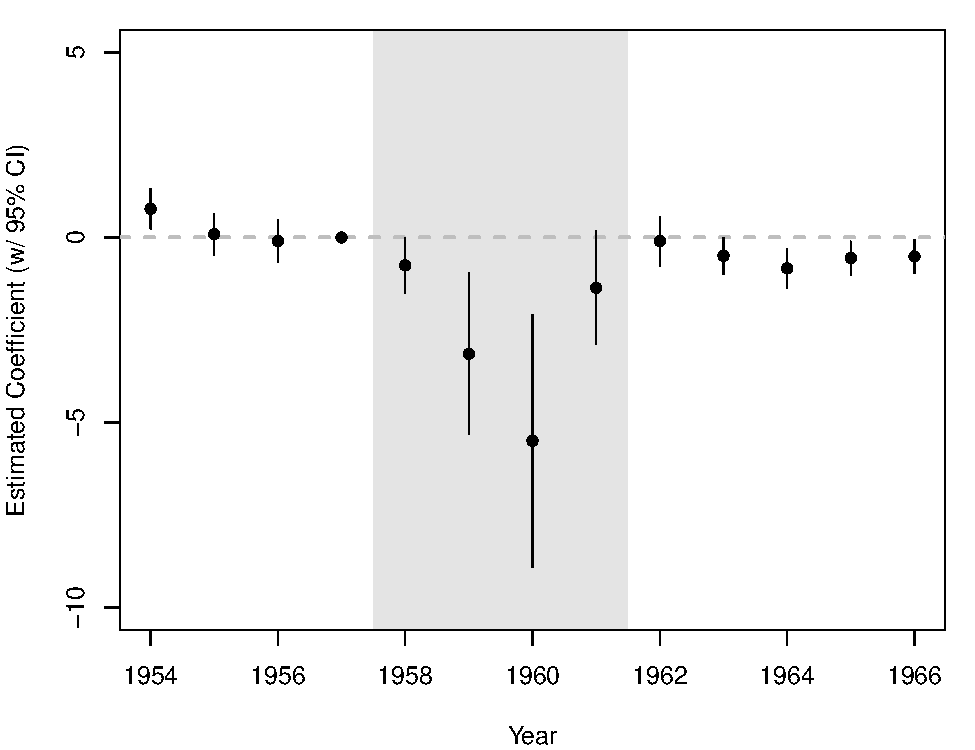
\includegraphics[width=\linewidth, height=0.62\textheight, keepaspectratio]{dyn_twfe1.pdf}
\end{column}
\begin{column}{0.49\textwidth}
\centering
\onslide<2->{{\small TWFE$^{*}$: additional interaction terms}\par\smallskip
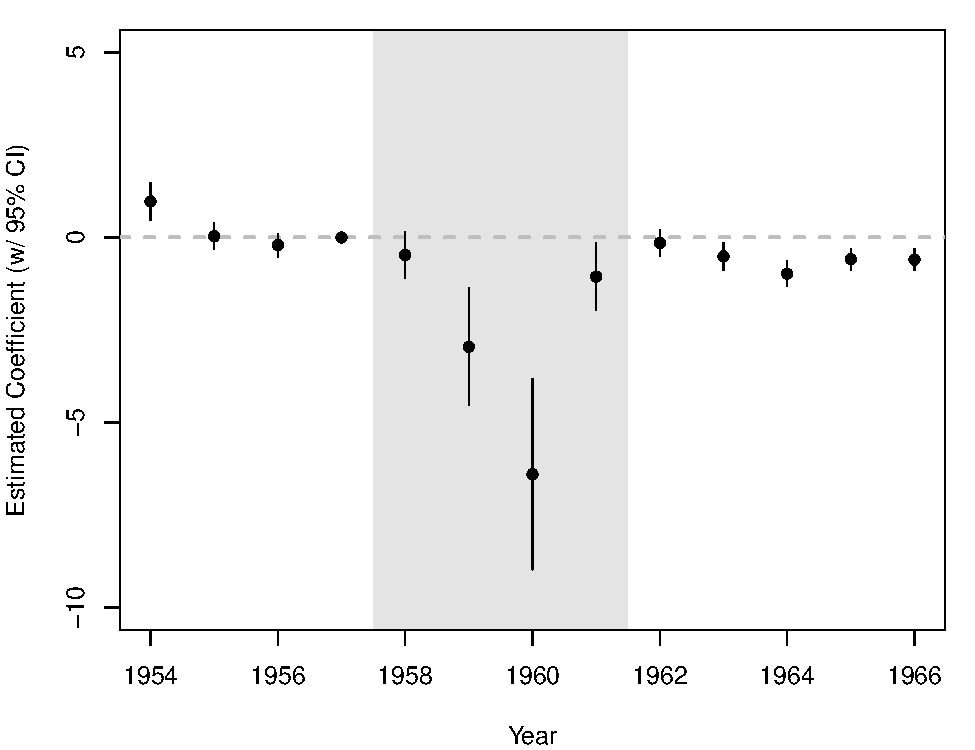
\includegraphics[width=\linewidth, height=0.62\textheight, keepaspectratio]{dyn_twfe2.pdf}}
\end{column}
\end{columns}
\end{frame}

\begin{frame}
  \frametitle{Dynamic Estimates: AIPW}
\begin{center}
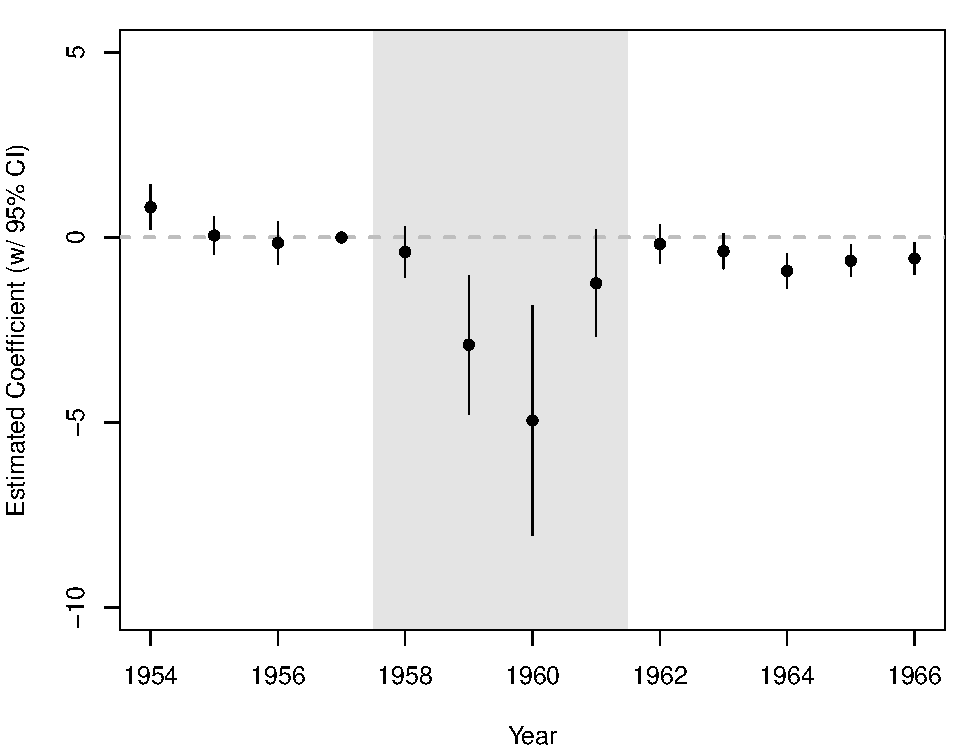
\includegraphics[height=0.74\textheight, keepaspectratio=1]{dyn_aipw.pdf}
\end{center}
\begin{itemize}
\item<2-> No visible pretrend; the mortality gap opens exactly in the famine years
\end{itemize}
\end{frame}

\begin{frame}
  \frametitle{Multi-valued $G$}
\begin{columns}[c,onlytextwidth]
\begin{column}{0.6\textwidth}
\centering
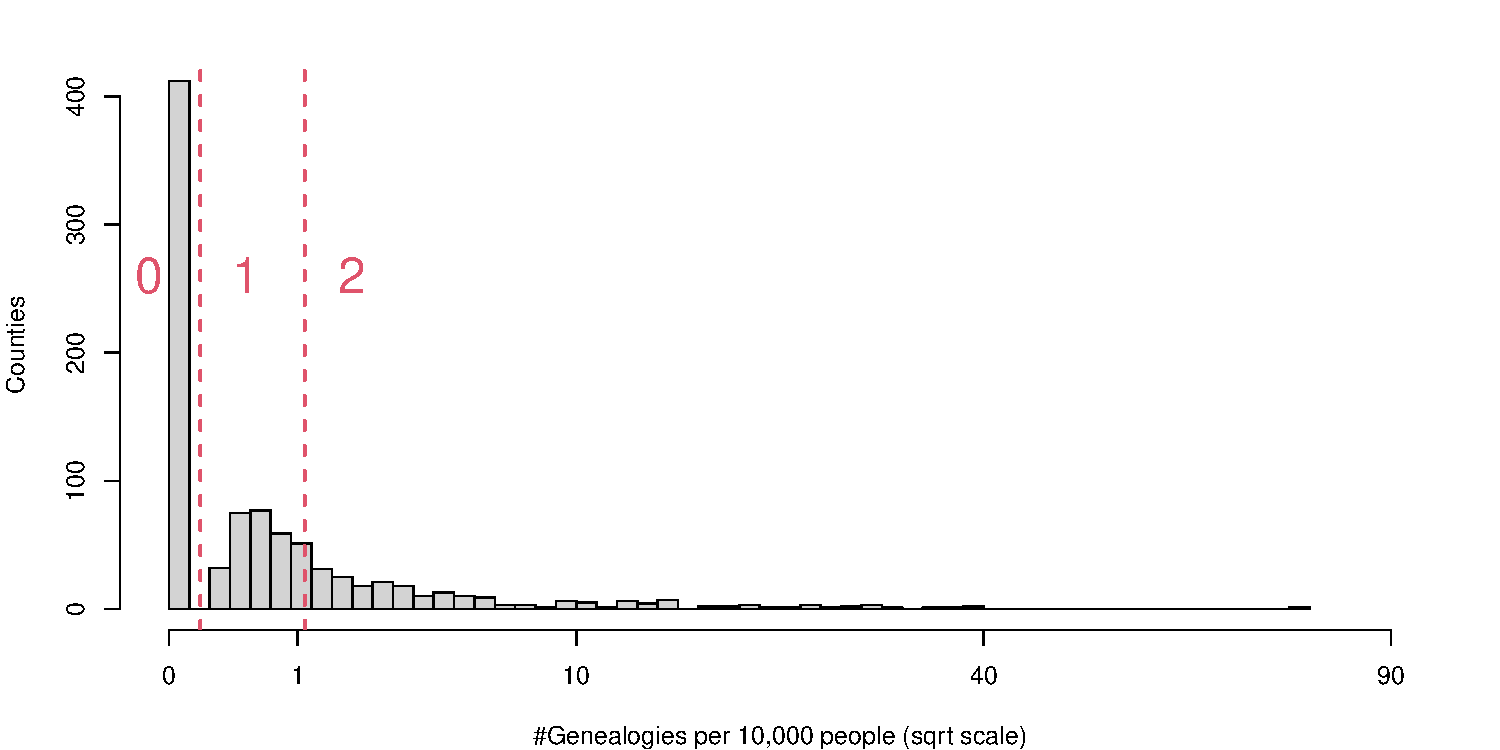
\includegraphics[width=\linewidth, height=0.66\textheight, keepaspectratio]{hist.pdf}
\end{column}
\begin{column}{0.37\textwidth}
\begin{itemize}\itemsep0.7em
\item $G=0$: 412 counties (no genealogies)
\item $G=1$: 254 counties (some genealogies)
\item $G=2$: 255 counties (many genealogies)
\end{itemize}
\end{column}
\end{columns}
\end{frame}

\begin{frame}
  \frametitle{Multi-valued $G$: AIPW Estimates}
\begin{columns}[T,onlytextwidth]
\begin{column}{0.49\textwidth}
\centering
{\small Group 0 vs Group 1}\par\smallskip
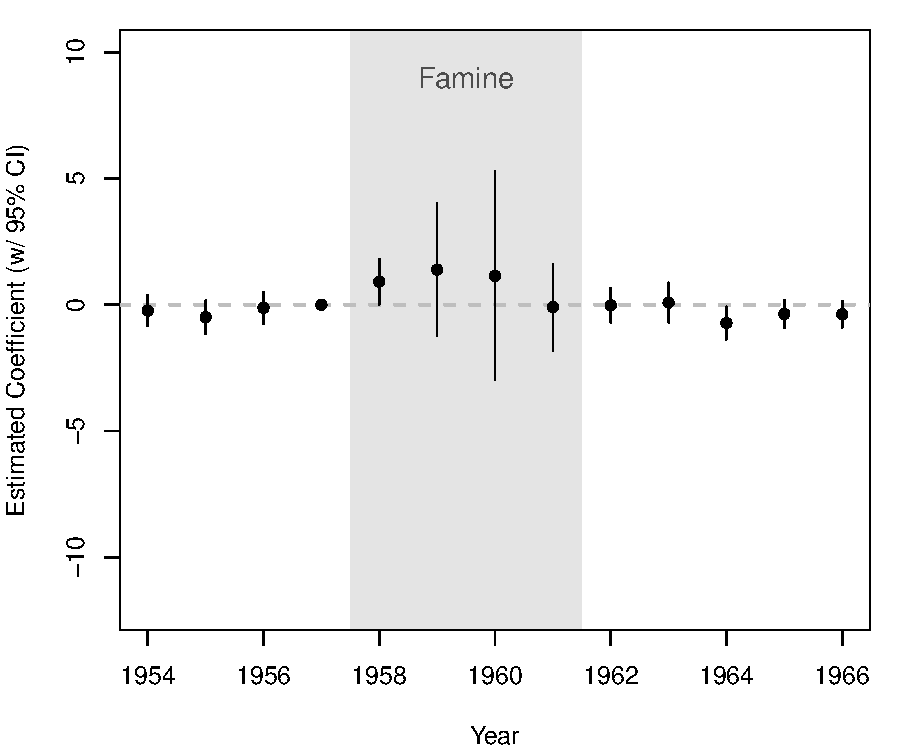
\includegraphics[width=\linewidth, height=0.62\textheight, keepaspectratio]{dyn_multi_low.pdf}
\end{column}
\begin{column}{0.49\textwidth}
\centering
\onslide<2->{{\small Group 0 vs Group 2}\par\smallskip
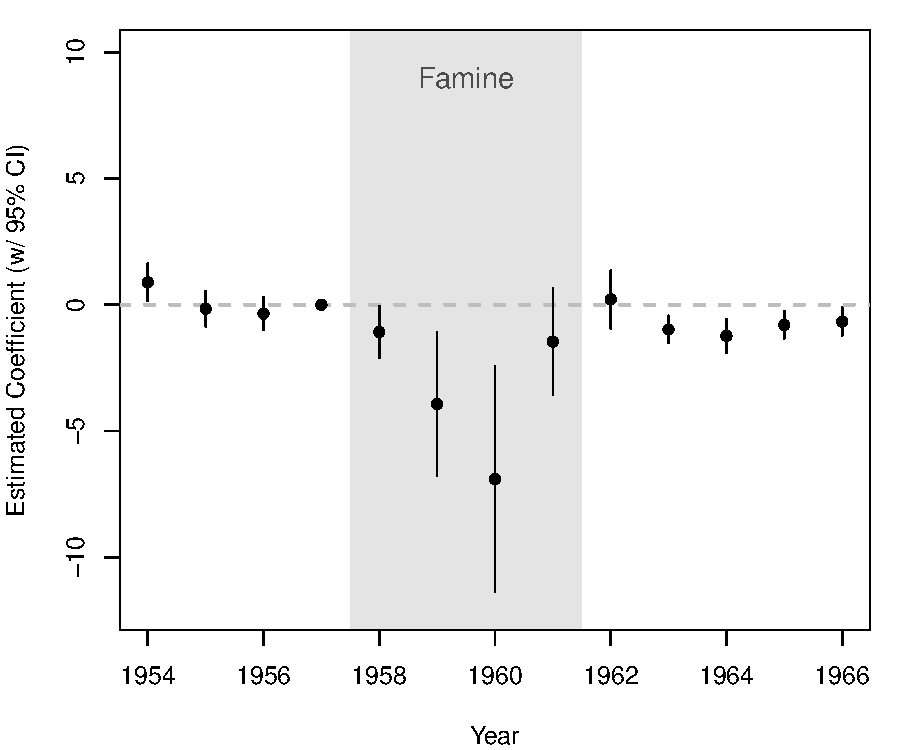
\includegraphics[width=\linewidth, height=0.62\textheight, keepaspectratio]{dyn_multi_high.pdf}}
\end{column}
\end{columns}
\begin{itemize}
\item<3-> The mortality gap concentrates where social capital is strongest
\end{itemize}
\end{frame}

\begin{frame}
  \frametitle{How to Correctly Interpret Your Findings?}
\begin{center}
\renewcommand{\arraystretch}{1.5}
\small
\begin{tabular}{p{0.2\textwidth}p{0.42\textwidth}p{0.3\textwidth}}
\textbf{Estimand} & \textbf{Interpretation in the running example} & \textbf{Key identifying assumptions} \\ \hline
\tem, effect modification & How did the average effect of exposure to famine on mortality differ between counties with high and low social capital? & No anticipation; parallel trends \\
\tatt, effect of exposure for $G=1$ & What was the average effect of exposure to famine on mortality in counties with high social capital? & $+$ exclusion restriction on $Z$ in group $G=0$ \\
\tcm, causal moderation & To what extent did high (vs. low) social capital mitigate the impact of famine on mortality? & No anticipation; parallel trends; $\red{\Delta Y(g,z) \indep G \mid X}$ \\
\tgz, $G$'s conditional effect & What was the average causal effect of social capital on mortality during the famine years? & $+$ exclusion restriction on $G$ absent the event \\ \hline
\end{tabular}
\end{center}
\end{frame}

\begin{frame}[fragile]
  \frametitle{FDID in R: The Famine Application}
\begin{columns}[T]
\column{.50\textwidth}
\begin{lstlisting}[language=R, basicstyle=\scriptsize\ttfamily, breaklines=true]
library(fdid)
mortality$any_gen <- as.integer(
  mortality$pczupu > 0)  # 412 vs 509 counties
s <- fdid_prepare(
  data = mortality,
  Y_label = "mortality",
  G_label = "any_gen",
  unit_label = "countyid",
  time_label = "year")

fit <- fdid(s, tr_period = 1958:1961,
            ref_period = 1957,
            method = "ols1")
\end{lstlisting}
\column{.46\textwidth}
\begin{block}{Observed interaction}
The famine $\times$ social-capital coefficient is an effect-modification contrast.
\end{block}
\begin{block}{Moderation interpretation}
Causal moderation requires factorial parallel trends.
\end{block}
\end{columns}
\end{frame}

\section{Conclusions}

\begin{frame}
  \frametitle{Practical Recommendations}
\begin{itemize}[<+->]\itemsep1.1em
\item What is your estimand?! {\small\parencite{lundberg2021what}}
\item Assess \underline{no anticipation} and \underline{parallel trends} (e.g., by checking pretrends)
\item If the goal is causal moderation, justify $\red{\Delta Y(g,z) \indep G \mid X}$ and show robustness of findings (e.g., by conducting sensitivity analysis)
\item If using TWFE models, demean covariates and add interaction terms $\red{G_i \cdot X_i \cdot \mathrm{Post}_t}$; check overlap
\item Should not automatically assume no carryover effects
\end{itemize}
\end{frame}

\begin{frame}
  \frametitle{Summary}
\begin{itemize}[<+->]\itemsep1.1em
\item When an event hits every unit, there is no untreated group; FDID compares before-after changes across levels of a \alert{baseline factor}
\item The arithmetic is canonical DID; the estimand is not: under no anticipation and parallel trends, $\tdid$ is \alert{effect modification} --- an associative quantity
\item \alert{Factorial parallel trends} ($\Delta Y(g,z) \indep G$) upgrades it to \alert{causal moderation}; an exclusion restriction on $G$ upgrades it to $G$'s conditional effect; an exclusion restriction on $Z$ recovers canonical DID
\item The broader lesson of these lectures: \alert{estimators are not research designs} --- the same arithmetic answers different questions under different assumptions
\item Lecture 4: back to TWFE regressions, and what breaks under staggered timing
\end{itemize}
\end{frame}

\begin{frame}
  \frametitle{Software}
\begin{itemize}\itemsep0.5em
\item \texttt{fdid} (R): factorial DID with the famine application data
\item \texttt{panelView} (R \& Stata): treatment status and outcome visualization
\item Tutorials: \url{https://yiqingxu.org/tutorials/panel.html}
\end{itemize}
\end{frame}

\appendix

\setbeamertemplate{frametitle continuation}[from second][(cont.)]
\begin{frame}[t,allowframebreaks=1.1]
  \frametitle{References}
  \referencelist
\end{frame}

\end{document}
